\documentclass[lettersize,journal]{IEEEtran}
\usepackage{amsmath,amsfonts}
\usepackage{amsmath}
\usepackage{algorithmic}
\usepackage{array}
\usepackage[caption=false,font=normalsize,labelfont=sf,textfont=sf]{subfig}
\usepackage{siunitx} 
\usepackage{textcomp}
\usepackage{booktabs}
\usepackage{mathtools}
\usepackage{stfloats}
\usepackage{url}
\usepackage{booktabs,multirow, threeparttable}
\usepackage{multicol}
\usepackage{lipsum}% http://ctan.org/pkg/lipsum
\usepackage{verbatim}
\usepackage{graphicx}
\usepackage{caption}
\usepackage{subcaption}
%\usepackage{subfigure}
%\usepackage{subfig}
\hyphenation{op-tical net-works semi-conduc-tor IEEE-Xplore}
\def\BibTeX{{\rm B\kern-.05em{\sc i\kern-.025em b}\kern-.08em
    T\kern-.1667em\lower.7ex\hbox{E}\kern-.125emX}}
\usepackage{balance}
\begin{document}
\title{Robust and Efficient CSI Compression Using CLLWCsiNet in Noisy MIMO Environments}

\author{
	\IEEEauthorblockN{Fardad Ansari\IEEEauthorrefmark{1}, Dr.Mahmood Mohassel Feghhi\IEEEauthorrefmark{2}}\\
	\IEEEauthorblockA{
		\IEEEauthorrefmark{1}Faculty of Electronic and Computer Engineering, 
		\IEEEauthorrefmark{2}Faculty of Electronic and Computer Engineering, 
	}\\
	\IEEEauthorblockA{
		\IEEEauthorrefmark{1}University of Tabriz, 
		\IEEEauthorrefmark{2}University of Tabriz, 
	}\\
	\IEEEauthorblockA{
		\IEEEauthorrefmark{1}f.ansari99@ms.tabrizu.ac.ir, \IEEEauthorrefmark{2}mohasselfeghhi@tabrizu.ac.ir
	}
}

\maketitle
\begin{abstract}
Multiple-Input Multiple-Output (MIMO) systems play a crucial role in advancing 5G and 6G networks by improving spectral efficiency and data rates. 
In Frequency Division Duplex (FDD) systems, since the channel reciprocity does not hold, timely feedback of Channel State Information (CSI) from receiver to transmitter is essential
to enable beamforming and precoding - which are fundamental techniques in MIMO systems. 
However, in massive MIMO configurations with large antenna arrays, this feedback mechanism introduces significant overhead to the system.
Among different compression methods, deep learning based approaches outperform traditional compressive sensing techniques, but 
their large parameter count poses challenges for deployment on resource-limited devices, such as user equipment. 
Moreover, factors such as short channel coherence time and imperfect wireless channels demand more robust models.
This paper introduces CLLWCsiNet (Convolutional Latent-space Low Weight CsiNet), a novel architecture that employs convolutional latent-space learning under imperfect channel conditions. CLLWCsiNet demonstrates superior predictive accuracy in noisy environments. 
We provide a comprehensive overview of previous models and introduce convolutional quantization techniques, which significantly reduce parameters and enhance computational efficiency. Our approach effectively compresses CSI while maintaining predictive accuracy, making it well-suited for deployment on resource-constrained user equipment.
Simulations show that CLLWCsiNet achieves -11 dB Normalized Mean Square Error (NMSE) in low SNRs (under 20 dB) with only 70K parameters. 
Additionally, we evaluate the proposed model on the Quadriga dataset for the first time, and demonstrating CLLWCsiNet's robust performance across varying noise levels.

\end{abstract}

\begin{IEEEkeywords}
Massive MIMO, CSI Feedback , deep learning, Convolutional Quantization,
Dynamic Quantization.
\end{IEEEkeywords}


\section{Introduction}
\label{sec:introduction}
Multiple-Input Multiple-Output (MIMO) systems play a pivotal role in the advancement of 5G and the forthcoming 6G networks by significantly enhancing spectral efficiency, data rates, and overall network capacity \cite{abc}. In Frequency Division Duplex (FDD) systems, where channel reciprocity is absent due to disjoint uplink and downlink frequency bands, accurate and timely feedback of Channel State Information (CSI) from the receiver to the transmitter becomes crucial for optimal performance. This feedback enables the transmitter to adapt its signaling strategies through precoding, beamforming, and rank adaptation, thereby improving link reliability and throughput. 

In Massive MIMO systems, the feedback overhead escalates with the growing number of antennas, necessitating efficient feedback mechanisms such as explicit (quantized CSI), implicit (codebook-based Precoding Matrix Indicator (PMI), Channel Quality Indicator (CQI), and Rank Indicator (RI)), and hybrid approaches. The downlink feedback is particularly vital, as it directly governs the base station's ability to exploit spatial multiplexing gains and mitigate multi-user interference. However, the feedback process introduces substantial overhead, which can degrade system efficiency if not managed properly. Therefore, studying and mitigating feedback overhead is essential to fully realize the benefits of MIMO technology in next-generation wireless communications (Figure \ref{csifeedbackimage}) \cite{abd}.

\begin{figure}[!t]
	\centering
	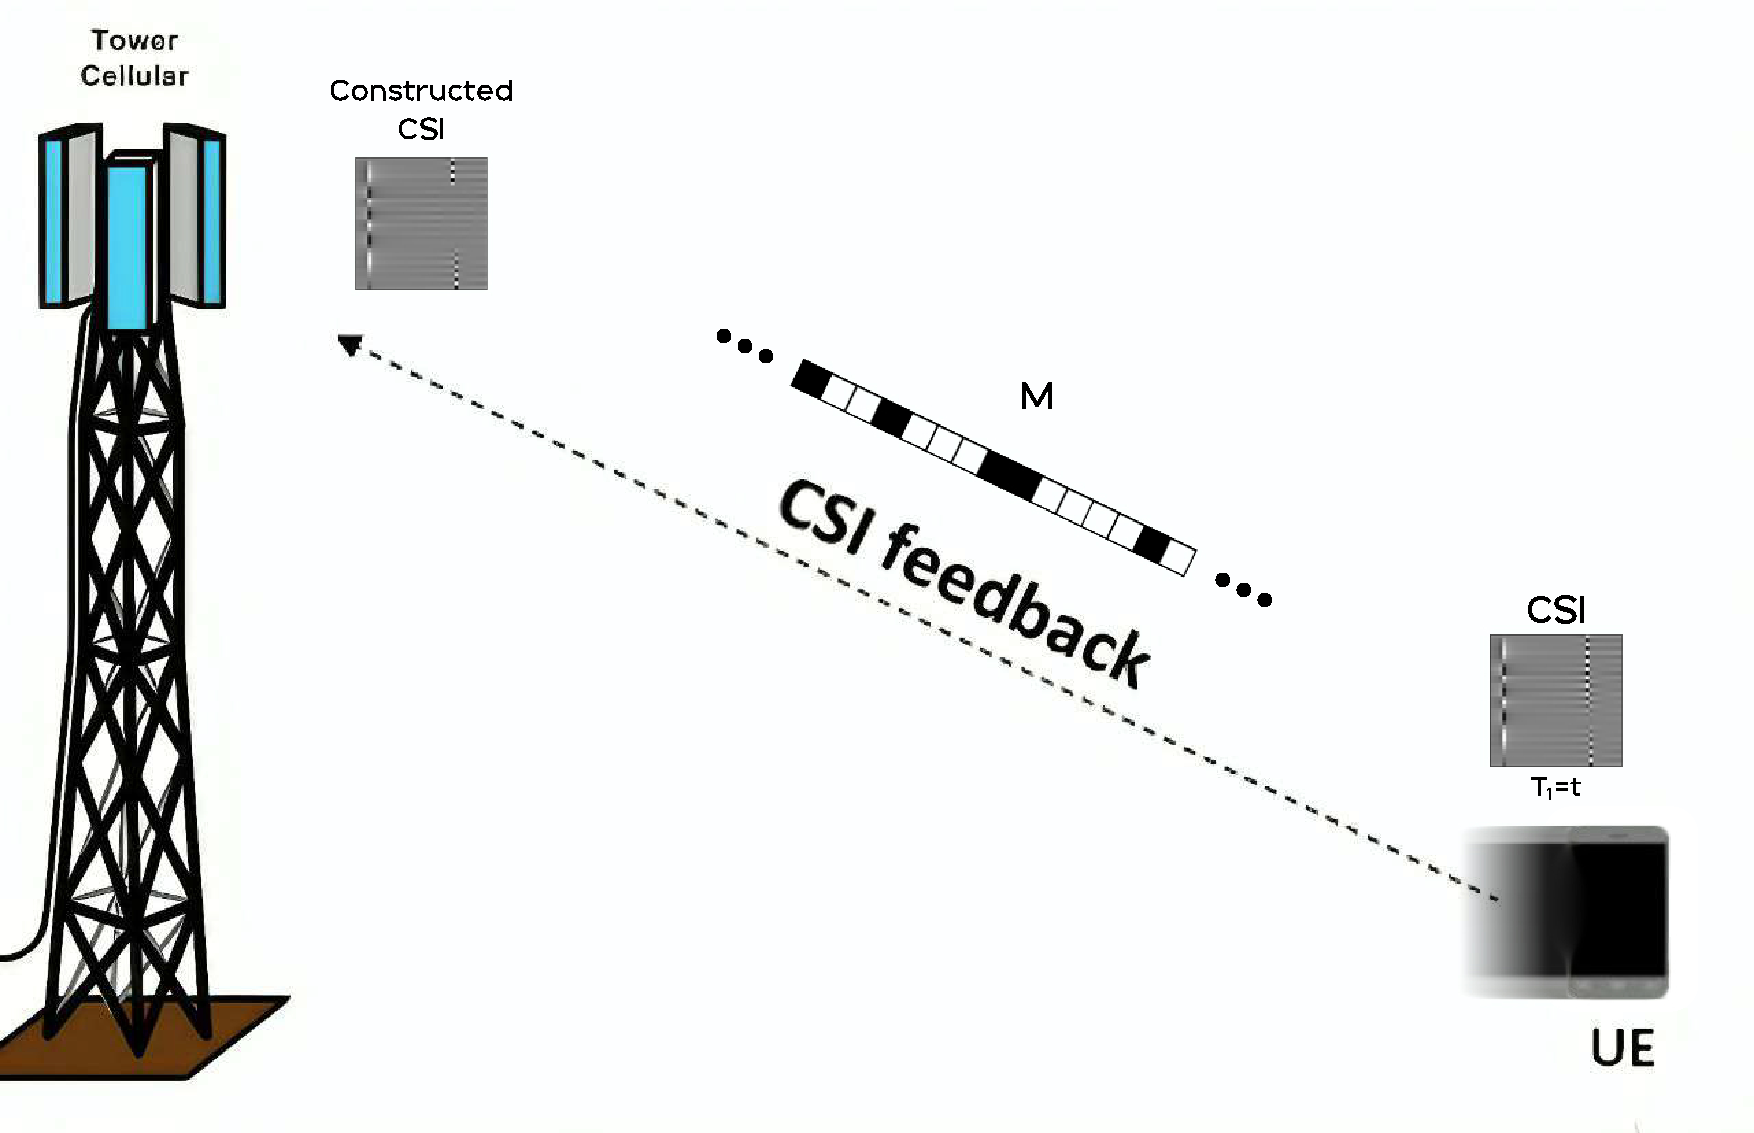
\includegraphics[width=2.5in]{BTS_User_Equipement.pdf}
	\caption{Downlink From UE to Base-Station}
	\label{csifeedbackimage}
\end{figure}

Efficient compression of Channel State Information (CSI) feedback has become a fundamental challenge in MIMO-FDD systems, driving innovations across signal processing and machine learning domains. Traditional compression methods, including scalar and vector quantization \cite{vectorquantiz}, Principal Component Analysis (PCA) \cite{pca}, and codebook-based techniques \cite{compressivesensing}, have established foundational approaches. While these methods provide computationally efficient solutions, they inherently face the accuracy-efficiency trade-off: scalar and vector quantization achieve dimensionality reduction through predefined level mapping, PCA preserves dominant orthogonal components, and standardized codebook methods (e.g., LTE) employ discrete codeword selection. However, such approaches often fail to adapt to the nonlinear, high-dimensional characteristics of modern wireless channels.

The limitations of conventional methods have spurred the adoption of deep learning architectures for CSI compression. Autoencoders now provide end-to-end learned representations through nonlinear latent space embedding, while recurrent neural networks (RNNs) explicitly model temporal channel correlations. Convolutional neural networks (CNNs) have proven particularly effective for massive MIMO by capturing spatial channel structures through hierarchical feature learning. Advanced paradigms like Variational Autoencoders (VAEs) introduce probabilistic encoding for noise resilience, and Generative Adversarial Networks (GANs) enable high-fidelity reconstruction through adversarial training. Emerging hybrid approaches combine these data-driven techniques with traditional compression principles, achieving superior performance by synergizing model-based and learning-based advantages. This evolution reflects the critical need for adaptive compression frameworks that balance reconstruction fidelity, computational complexity, and feedback overhead in next-generation networks.


\subsection{Related Work}
Pioneering the application of deep learning to CSI feedback compression, Wen et al. \cite{abe} introduced an auto-encoder architecture. This seminal work laid the groundwork for extensive subsequent research that explored the integration of wireless communication system dynamics within MIMO systems using auto-encoder frameworks. In this initial setup, the encoder emulated the user equipment, while the decoder functioned at the receiver. The inherent randomness of channel state information was simulated using the COST2100 channel model \cite{abf}, leading to the creation of the corresponding COST2100 dataset.

Building upon this foundation, numerous architectures, predominantly based on auto-encoders, have been proposed. Wen et al. further developed this line of research with CsiNet \cite{abe}, an autoencoder notable for incorporating the Residual Network concept \cite{abg} within its decoder. Addressing the temporal aspects of wireless channels affected by user mobility, Wang et al. \cite{abh} introduced time-varying CSI Feedback by integrating Long Short-Term Memory (LSTM) units into the decoder of an auto-encoder. Lu et al. \cite{abi} expanded on this by implementing LSTM in both the encoder and decoder of their model. However, their choice of a fully connected network for LSTM, instead of a convolutional structure, reportedly doubled the parameters and complexity compared to CsiNet-LSTM \cite{abh}. Their proposed RecCsiNet \cite{abi} prioritized memory for feature extraction over direct correlation, employing LSTM in parallel with a fully connected layer, similar to skip connections in residual networks \cite{abi}, achieving superior performance before considering temporal correlation by applying LSTM to residual features rather than correlation features \cite{abh}.

Further refining these approaches, Mashhadi et al. \cite{mashhadi2020deepcmc} introduced DeepCMC, a fully convolutional neural network where dimensional compression is achieved through pooling layers. To enhance compression, they also employed context-adaptive binary arithmetic coding on the encoder's output. Shehzad et al. \cite{shehzad2021design} proposed a novel machine learning-based approach utilizing twin recurrent neural networks at both the base station and user equipment to reduce CSI feedback overhead while maintaining accuracy. Zhang et al. \cite{zhang2022quantization} tackled the critical issue of quantization in DL-based CSI feedback by proposing an adaptor-assisted quantization strategy to improve feedback efficiency and accuracy. Liu et al. \cite{liu2023continuous} addressed the challenge of performance degradation due to distribution shifts by proposing a continuous online learning framework to maintain accuracy across diverse channel conditions. Guo et al. \cite{guo2023ris} introduced RIS-CoCsiNet, a cooperative CSI feedback framework for RIS-assisted systems, separating RIS-UE CSI into shared and unique components and achieving significant NMSE improvements through magnitude-dependent phase feedback strategies.

More recent advancements continue to push the boundaries of DL-based CSI feedback. Li and Wu \cite{abj} extended the RecCsiNet model by decoupling feature extraction from compression and decompression, resulting in their Convlstm model, which reportedly significantly reduced error \cite{abj}. Liu et al. \cite{abk} also focused on coherence time simulation with LSTM and introduced Markovenet, featuring a novel convolutional latent space that reduces model parameters and complexity. They argued for the superiority of convolutional approaches over fully connected layers for feature extraction in CSI matrices due to the localized correlations. Lu et al. \cite{abn} presented CRNet, a significant early work employing small kernel sizes for fine-grained feature extraction and utilizing a residual network in both encoder and decoder with multi-resolution blocks. Guo et al. \cite{abo} proposed a multiple-rate architecture (CsiNetPlus), incorporating non-uniform quantization and larger kernel sizes to dynamically adjust compression ratios based on the environment without retraining. Yu et al. \cite{abq} explored the use of non-local blocks, drawing inspiration from sequence denoising work \cite{abr}, to capture long-range dependencies and enhance accuracy. Cai et al. \cite{abs} introduced Attention-CsiNet, replacing fully connected layers with LSTMs for sub-carrier coherence extraction and incorporating an attention module inspired by machine translation research \cite{abt}. Liang et al. \cite{abm} proposed CSRenet, a compressive sensing architecture combining compressive sensing at the encoder with deep learning at the decoder.

Continuing this trend of innovation, recent studies in 2024 have further refined DL-based CSI feedback techniques. Wang et al. \cite{wang2024better} introduced a novel test channel-based quantization module (TCQM) to address limitations in existing systems. Zhang et al. \cite{zhang2024zone} proposed a zone-specific deep learning approach, training specialized autoencoders for different spatial zones to account for varying channel characteristics. Chen et al. \cite{chen2024transnet} presented TransNet+, an enhanced Transformer-based architecture leveraging higher-dimensional features and an optimized multi-head attention mechanism, achieving superior performance, especially at high compression ratios. Li et al. \cite{li2024lightweight} proposed GCRNet, a Ghost module-based architecture that reduces feature redundancy, achieving comparable accuracy to prior work with significantly lower complexity \cite{ji2021clnet}. Wang et al. \cite{wang2024variational} introduced a variational autoencoder framework for noisy channels, optimizing rate-distortion and demonstrating robustness across different SNRs. Ma et al. \cite{Ma2024} presented Csi-L2O, a learning-to-optimize framework combining compressive sensing and deep learning, achieving state-of-the-art performance with significantly reduced encoder complexity. Lu et al. \cite{prac2024} identified challenges like channel distribution shifts and proposed an alternating optimization framework with online knowledge review to enhance adaptability, demonstrating substantial NMSE improvements in unseen environments. Yin et al. \cite{quant2024} proposed a dynamic bit allocation strategy for encoder outputs, jointly optimizing quantization codebooks and autoencoder weights to reduce NMSE. \cite{CSICompression2024} provided a comprehensive analysis of CSI feedback overhead and a comparison of traditional and data-driven approaches, highlighting trade-offs for 5G-Advanced deployment. Finally, \cite{Guo2024} introduced a one-sided CSI-PPPNet architecture with a joint multi-module learning framework, significantly reducing parameters and improving spectral efficiency by simultaneously optimizing feedback, coding, and precoding modules.
Before presenting our solution, we first analyze the fundamental limitations of existing approaches.

\subsection{Key Challenges in CSI Feedback Compression}
The design of efficient CSI feedback systems must balance three critical constraints: 
\begin{itemize}
    \item \textbf{Computational Complexity}: Most auto-encoder architectures (e.g., CsiNet \cite{abe}) rely heavily on fully connected layers, which account for over 99\% of parameters (2.1M) and 37\% of FLOPs (5.6M). Our analysis shows that simply removing these layers reduces parameters to 3,400 (-99.8\%) and FLOPs to 3.5M (-37.5\%), but at the cost of degraded accuracy.
    
    \item \textbf{Kernel Size Sensitivity}: The choice of convolutional kernel sizes significantly impacts resource usage. For instance, increasing kernel size from (3,3) to (7,7) in CsiNet \cite{abe} raises FLOPs by 362\% (to 20.3M) with only a 1.44\% parameter increase, highlighting the need for careful architecture design.
    
    \item \textbf{Hardware Limitations}: As shown in Table~\ref{table:methods_params}, state-of-the-art models like TransNet \cite{abz} require 50M+ FLOPs and 2.38M parameters - impractical for UE devices with limited GPU power and storage.
\end{itemize}
These challenges motivate our proposed architecture in Section~\ref{sec:proposed_model}, which achieves sub-100K parameters while maintaining competitive NMSE.


\begin{table}[htb]
	\centering
	\caption{Methods Parameters}
	\label{table:methods_params}
	\begin{tabular}{ c|cc }
		\hline
		\multicolumn{1}{c|}{Methods}      & \multicolumn{2}{c}{Params}     \\
		& \multicolumn{1}{c}{UE Params}             & \multicolumn{1}{c}{UE FLOP} \\
		\hline
		CsiNet     & 1052K      & 1094k \\
		CRNet        & 1049K      & 1235K \\
		ACRNet-1x    & 1049K      & 1235K \\
		CsiNetPlus   & 1049K      & 1462K \\
		TransNet     & 2381K      & 1054K \\
		\hline
	\end{tabular}
\end{table}


\subsection{Contributions}

In this paper, we address the inefficiencies associated with the fully connected layers in many state-of-the-art models for CSI feedback compression. These layers often propagate redundant weights related to the zero parts of the channel state information, leading to a large number of parameters. This inefficiency is particularly problematic on User Equipment (UE), where resource constraints such as memory and computational power are critical factors. By focusing on quantization techniques, we aim to significantly reduce the parameter count and enhance the efficiency of CSI feedback compression models on UE.

We retrained the previously proposed models with a convolutional latent space on the COST2100 dataset \cite{abf}, revealing that many designs fail in the absence of fully connected layers. To overcome this, we proposed a new architecture named CLLWCsiNet (Convolutional Latent-space Low-weight CsiNet), which achieves high accuracy without relying on fully connected layers and performs better with significantly fewer parameters. Furthermore, to ensure generalization, we evaluated these models on the Quadriga dataset \cite{abt}, specifically generated for outdoor scenarios. Notably, many models that exhibited high accuracy on the COST2100 dataset \cite{abf} failed when tested on the Quadriga dataset\cite{abt}.

Our study also considers the imperfect channel conditions, a realistic scenario often neglected in favor of ideal conditions in wireless communication systems research. The proposed CLLWCsiNet model demonstrated performance comparable to CsiNet+DNNet \cite{abw}, which has a significantly higher number of parameters. Importantly, CLLWCsiNet maintained high accuracy across varying noise power levels, showcasing robust performance. For the first time, we employed quantization not merely for fully connected layers or bit stream generation but also within the convolutional framework. This novel application of quantization is crucial for practical deployments, as it significantly reduces the computational burden and memory requirements, making the models more suitable for resource-constrained environments typical of wireless communication systems.

The importance of quantization in this context cannot be overstated. It allows for the compression of model parameters without significant loss of accuracy, facilitating the deployment of deep learning models in real-time and low-power scenarios. Models with a high number of parameters, while potentially more accurate, often face practical limitations in wireless communication systems due to their substantial resource demands, including computational power and energy consumption. By incorporating convolutional quantization, our proposed CLLWCsiNet model addresses these challenges, offering a more efficient and scalable solution for CSI feedback compression in next-generation wireless networks.

The following is a list of the contributions:

\begin{itemize}
	\item To the best of our knowledge, this is the first time that dynamic quantization has been explicitly applied to all layers of a neural network for CSI compression tasks. Previous research has primarily focused on network binarization in fully connected layers within the latent space, aiming to enable quantization from a communication system design perspective. However, this concept can be extended to all layers, which can significantly reduce network complexity, albeit potentially at the expense of accuracy.
	
	Bit-level neural networks are a crucial subset of network quantization, enabling the deployment of deep learning models on devices with constrained resources, such as those found in wireless communication systems. It is important to distinguish between network quantization and codeword quantization, which involves larger compression representations as proposed in communication system designs.
	
	
	\item Unlike most research in this domain, our focus is on imperfect channels characterized by additive white Gaussian noise (AWGN) in wireless communication systems. Previous studies that consider imperfect channels include \cite{abw} and \cite{abs}. In \cite{abw}, a DNNet was proposed, which introduces high complexity even in low dimensions, despite the training process being conducted in two stages. Researchers in \cite{abs} proposed a variational auto-encoder for imperfect channels, but they did not report numerical results. In contrast, we propose a fully convolutional neural network (CNN) with a latent space alongside a simple subtraction denoising convolution filter for stabilizing accuracy and denoising, respectively. Our architecture is trained in a single stage, unlike the approach in \cite{abw}. Our results demonstrate the state-of-the-art performance of this denoising network compared to \cite{abw}.
	
	\item We propose a convolutional latent space low-light CSINet named CLLWCsiNet, which achieves high accuracy compared to architectures that use fully connected layers. Previous architectures rely heavily on fully connected layers, which introduce redundant zero weights and significantly increase the model's parameter count by approximately 2 million parameters. This increase in parameters leads to high computational costs Floating Point Operations (FLOPs) and storage requirements, making them impractical for user equipment with limited GPU power and storage capacity, especially in scenarios involving low temporal CSI information and CPU-based mass-produced user devices. Furthermore, most of these architectures are designed under ideal channel conditions.

	
	
	
\end{itemize}


\section{System Model}
\label{sec:system_model}

\subsection{System Configuration}
While our system model adopts Rayleigh fading for tractability in theoretical analysis, the training data (COST 2100) captures more realistic propagation effects, including spatial consistency and clustered multipath. This hybrid approach allows us to benchmark against classical Rayleigh-based systems while ensuring the model learns robust features from real-world channel characteristics. We note that Rayleigh fading serves as a lower-bound baseline, and the model’s performance on COST 2100 (and Quadriga) reflects its capability in practical scenarios.
Like most scenarios adopts a single user massive MIMO system in a single cell, in which the base station equips $N_{t} > 1$ transmitting antennas as well as the UE with a single receiving antennas. An orthogonal frequency division multiplexing (OFDM) system with $N_{c}$ sub-carriers for FDD downlink massive MIMO is examined. In the OFDM-MIMO system considered in this work, the subcarriers are assumed to maintain orthogonality.

\subsection{Channel Model}
The time-domain channel impulse response between the $i$-th transmit antenna and UE follows Rayleigh fading:
\[
h_i(\tau) = \sum_{l=1}^L \alpha_{i,l} \delta(\tau-\tau_l), \quad \alpha_{i,l} \sim \mathcal{CN}(0,\sigma_l^2)
\]
where:
\begin{itemize}
    \item $h_i(\tau)$ is the time-domain channel impulse response for antenna $i$
    \item $\alpha_{i,l}$ is the complex gain of the $l$-th path (Rayleigh distributed)
    \item $\tau_l$ is the delay of the $l$-th path
    \item $L$ is the total number of multipath components
    \item $\mathcal{CN}(0,\sigma_l^2)$ denotes complex Gaussian distribution with variance $\sigma_l^2$
\end{itemize}
The frequency-domain channel matrix for subcarrier $n$ is:
\[
\mathbf{H}_n = \left[H_{1,n}, H_{2,n}, \dots, H_{N_t,n}\right] \in \mathbb{C}^{1 \times N_t}
\]
where:
\begin{itemize}
    \item $\mathbf{H}_n$ is the frequency-domain channel matrix for subcarrier $n$
    \item $H_{i,n}$ is the channel coefficient for antenna $i$ and subcarrier $n$
    \item $N_t$ is the number of transmit antennas
\end{itemize}
with elements derived from:
\[
H_{i,n} = \sum_{l=1}^L \alpha_{i,l} e^{-j2\pi n \tau_l/N_c}
\]



\subsection{Pilot Transmission}
We will assume base station sends orthogonal pilots for each subcarrier to the UE $n=1,...,N_{c}$: let pilot matrix $\mathbf{X}_{p,n}\in \mathbb{C}^{N_{t}\times T_{p}}$ be orthogonal ($T_{p} \geq N_{t}$). We will assume on $n^{th}$ sub-carriers the received signal at UE will be equal to: 
\[
\mathbf{Y}_{p,n}=\mathbf{H}_{n}\mathbf{X}_{p,n}+\mathbf{Z}_{n} 
\]
where $\mathbf{Y}_{p,n} \in \mathbb{C}^{1\times T_{p}}$ ($N_{r}=1$) is received pilot at $n^{th}$ subcarrier, $\mathbf{H}_{n} \in \mathbb{C}^{1\times N_{t}}$ is the MIMO channel matrix for subcarrier $n$ and $\mathbf{Z}_{n}\in \mathbb{C}^{1\times T_{p}}$ is AWGN noise with variance $\sigma^{2}$.

\subsection{Channel Estimation}
Let's assume UE uses Least Squares (LS) to estimate $\mathbf{H}_{n}$:
\[
\hat{\mathbf{H}}_{n}=\mathbf{Y}_{p,n}\mathbf{X}^{\dag}_{p,n}
\]
where $\hat{\mathbf{H}}_{n} \in \mathbb{C}^{1\times N_{t}}$ and $\mathbf{X}_{p,n}^{\dag}= \mathbf{X}^{H}_{p,n}(\mathbf{X}_{p,n}\mathbf{X}^{H}_{p,n})^{-1}$. The pilot matrix $\mathbf{X}_{p,n}$ satisfies $\mathbf{X}_{p,n} \mathbf{X}_{p,n}^H = \mathbf{I}_{N_t}$ for $T_p \geq N_t$.

\subsection{CSI Feedback}
For each subcarrier estimated CSI matrices is $\{ \hat{\mathbf{H}}_{1},...,\hat{\mathbf{H}}_{N_{c}} \}$. For simplicity we stack and reshape the channel matrix into:
\[
H_{\text{freq}}=\left[\hat{\mathbf{H}}_{1}^{H},\hat{\mathbf{H}}_{2}^{H},...,\hat{\mathbf{H}}_{N_{c}}^{H}\right]^{H}_{N_{c}\times N_{t}}
\]
$H_{\text{freq}} \in \mathbb{C}^{N_c \times N_t}$ is the stacked CSI matrix across subcarriers. Evidently, $H_{\text{freq}} \in \mathbb{C}^{N_{c}\times N_{t}}$ has $2\times N_{c}\times N_{t}$ float numbers, which is too big for direct feedback in a massive MIMO system and this feedback is required for creating the precoding to be built by base station.

$H_{\text{freq}}$ is the spatial-frequency domain equivalent of the CSI. We use the 2D discrete Fourier transform (DFT) and transfer $H_{\text{freq}}$ into the angle-delay domain as follows to extract the CSI features:
\[
\tilde{\mathbf{H}} = \mathbf{F}_d H_{\text{freq}} \mathbf{F}_a^H
\]
where $\mathbf{F}_d \in \mathbb{C}^{N_{c}\times N_{c}}$ is delay DFT and $\mathbf{F}_a \in \mathbb{C}^{N_{t}\times N_{t}}$ is angular DFT and both of them are unitary DFT matrices.

CSI shows sparsity in the delay domain, with $\tilde{\mathbf{H}}$ having significant values only in the first $N_{i}$ rows because the time of arrival (TOA) between multipaths is limited in duration. Like aforementioned researches, we select first $N_{i}$ rows of $\tilde{\mathbf{H}}$ to create a new channel matrix $\tilde{\mathbf{H}}_f$ as
\[
\tilde{\mathbf{H}}_f = \left[ \tilde{\mathbf{H}} \right]_{1:N_{i}} 
\]

$\tilde{\mathbf{H}}_f$ as is still too heavy for feedback, though, because in a massive MIMO system, $N_{t}$ is a big number. Our goal is to further compress matrix $\tilde{\mathbf{H}}_f$ in order to minimize the weight of the feedback.

\subsection{Deep Learning Compression}
In an effort to lower transmission overheads, DL-based algorithms have recently been used in CSI feedback. An encoder at UE first compresses the CSI data into a codeword:
\[
s = f_{\text{enc}}(\tilde{\mathbf{H}}_f) 
\]
and after that, a feedback channel is used to send the codeword to the BS. A decoder at the BS can recreate the CSI as:
\[
\hat{\tilde{\mathbf{H}}}_f = f_{\text{dec}}(s) 
\]

The reconstruction quality is evaluated using the Normalized Mean Square Error (NMSE):
\[
\text{NMSE} = \mathbb{E}\left\{\frac{\|\tilde{\mathbf{H}}_f - \hat{\tilde{\mathbf{H}}}_f\|_F^2}{\|\tilde{\mathbf{H}}_f\|_F^2}\right\},
\]
where $\|\cdot\|_F$ denotes the Frobenius norm and $\mathbb{E}\{\cdot\}$ represents expectation over the dataset.

The compression ratio can be obtained as:
\[
\gamma = \frac{N_{s}}{2\times N_{i}\times N_{t}}  
\]
where $\gamma$, $N_{s}$, $N_{i}$ and $N_{t}$ are compression ratio, codeword length, selected rows from $\tilde{H}$ and number of transmit antenna.

\subsection{End-to-End Effective SNR Analysis}
The effective SNR at the receiver accounts for both channel estimation and compression errors. Let $\mathbf{H} \in \mathbb{C}^{N_c \times N_t}$ denote the true channel matrix, and $\hat{\mathbf{H}} = \mathbf{H} + \mathbf{E}_{\text{est}}$ its estimate from pilot symbols, where $\mathbf{E}_{\text{est}}$ is the estimation error matrix with i.i.d. elements $\sim \mathcal{CN}(0,\sigma_{\text{est}}^2)$. After compression/decompression, the reconstructed channel becomes:

\begin{equation}
\hat{\tilde{\mathbf{H}}}_f = \tilde{\mathbf{H}}_f + \mathbf{E}_{\text{comp}}, \quad \mathbf{E}_{\text{comp}} \sim \mathcal{CN}(0,\sigma_{\text{comp}}^2)
\end{equation}

The \textbf{effective SNR} for data detection is derived as:

\begin{equation}
\text{SNR}_{\text{eff}} \coloneqq \frac{\mathbb{E}\{\|\mathbf{H}\|_F^2\}}{\mathbb{E}\{\|\mathbf{E}_{\text{total}}\|_F^2\}} = \frac{N_t N_c P}{\sigma_{\text{est}}^2 + \sigma_{\text{comp}}^2 + N_0}
\end{equation}

\noindent where:
\begin{itemize}
\item $P$ is the transmit power per subcarrier
\item $\sigma_{\text{est}}^2 = \frac{N_0}{T_p E_p}$ is the pilot-based estimation error variance ($T_p$: pilot length, $E_p$: pilot energy)
\item $\sigma_{\text{comp}}^2 = \|\mathbf{F}_a\|^2 \cdot 10^{\text{NMSE}/10} \cdot P$ converts NMSE to compression error power
\item $N_0$ is the thermal noise density
\end{itemize}

For orthogonal pilots with $T_p \geq N_t$, this simplifies to:

\begin{equation}
\text{SNR}_{\text{eff}} = \frac{N_t \gamma}{1 + \gamma\left(\frac{1}{\beta} + 10^{\text{NMSE}/10}\right)}, \quad \text{where } \gamma \coloneqq \frac{P}{N_0}
\end{equation}

\noindent and $\beta \coloneqq T_p E_p/N_0$ is the pilot SNR. 


\subsection{Mathematical Modeling of Feedback Imperfections}
\label{subsec:feedback_noise}

This analysis focuses exclusively on imperfections introduced \textit{during} the feedback transmission, assuming perfect channel estimation and compression at the UE. The two-stage noise model is:

\subsubsection{Noiseless Compression}
At the UE, the CSI matrix $\mathbf{H}_f$ is perfectly compressed to a codeword:

\begin{equation}
    \mathbf{s} = f_{\text{enc}}(\mathbf{H}_f)
\end{equation}

where $f_{\text{enc}}$ represents the ideal compression function.

\subsubsection{Feedback Channel Corruption}
During uplink transmission, the codeword is corrupted by AWGN:

\begin{equation}
    \tilde{\mathbf{s}} = \mathbf{s} + \mathbf{n}, \quad \mathbf{n} \sim \mathcal{CN}(0,\sigma_n^2\mathbf{I})
    \label{eq:noisy_feedback}
\end{equation}

with noise power $\sigma_n^2$ calculated from the uplink SNR:

\begin{equation}
    \sigma_n^2 = \frac{\mathbb{E}[\|\mathbf{s}\|_2^2]}{N_s \cdot 10^{\text{SNR}_{\text{dB}}/10}}
\end{equation}

where $N_s$ is the codeword length.

\subsubsection{Denoising and Reconstruction}
The BS applies a denoising operator $\mathcal{D}$ to obtain:

\begin{equation}
    \hat{\mathbf{s}} = \mathcal{D}(\tilde{\mathbf{s}})
\end{equation}

followed by ideal reconstruction:

\begin{equation}
    \hat{\mathbf{H}}_f = f_{\text{dec}}(\hat{\mathbf{s}})
\end{equation}

\subsubsection{Error Decomposition}
The total NMSE contains only feedback-induced errors:

\begin{equation}
    \text{NMSE} = \underbrace{\frac{\mathbb{E}[\|\mathbf{H}_f - f_{\text{dec}}(\mathbf{s})\|_F^2]}{\|\mathbf{H}_f\|_F^2}}_{\text{Compression error}} + \underbrace{\frac{\mathbb{E}[\|f_{\text{dec}}(\mathbf{s}) - f_{\text{dec}}(\hat{\mathbf{s}})\|_F^2]}{\|\mathbf{H}_f\|_F^2}}_{\text{Denoising error}}
\end{equation}

\begin{itemize}
    \item \textbf{Key Assumption}: Channel estimation errors and pre-compression noise are negligible ($\mathbf{H}_f$ is perfect)
    \item \textbf{Scope}: All noise enters through the feedback channel (\eqref{eq:noisy_feedback})
\end{itemize}

\section{Analysis of Existing Denoising Approaches}
\subsection{DNNet Architecture Breakdown}

Sun et al. \cite{bbb1} acknowledge the presence of imperfect channels. However, there exists a discrepancy between the imperfect channel and their suggested model. They do not account for the imperfect channel during the feedback transmission process. Instead, they attempt to mitigate noise from the channel state information matrix by employing a denoising module at the frontend before generating the codeword and prior to entering the decoder. This approach may not fully capture the complexities of real-world channel imperfections and could potentially lead to suboptimal performance in practical scenarios.
Ye and colleagues \cite{abw} address the challenge of imperfect channels by proposing the DNNet, drawing inspiration from DNCNN \cite{ccc1}. Their denoising module is designed to seamlessly integrate with various auto-encoders such as CsiNet \cite{abe}, CRNet \cite{abn}, and ACRNet \cite{aby}.
The proposed algorithm of DNNet can be outlined as follows:
DNNet comprises a Noise Extraction Unit (NEU), designed to extract noise from the codeword. This noise is then subtracted from the noisy codeword using one input layer, one output layer, and 
\begin{math} \ L-2 \end{math} hidden layers. Both the input and output layers maintain the same dimensions as the compressed codewords. Let suppose the generated codeword by encoder part of CsiNet is :

\begin{equation}
%	\begin{math}
		S=[s_{1},s_{2},s_{3},...,s_{cw}]
%	\end{math}
\end{equation}

After adding additive Gaussian noise to the codeword the noisy codeword is as follow:

\begin{equation}
%	\begin{math}
		\tilde{S}=S+\textbf{n}
%	\end{math}
\end{equation}



\begin{equation}
%	\begin{math}
		\tilde{S}=[\tilde{s}_{1},\tilde{s}_{2},\tilde{s}_{3},...,\tilde{s}_{cw}]
%	\end{math}
\end{equation}

And then this codeword is input layer of DNNet. The output of NEU is the noise that is extracted from codeword:

\begin{equation}
%	\begin{math}  
		\tilde{n}=g_{L}(...g_{1}(\tilde{S})) 
%		\end{math}
\end{equation}

The structure of proposed DNNet is as follows for each \textit{lth} 
layer:

\begin{equation}
\left\{
\begin{array}{ll}
	z  & \mbox{if } l=1 \\
	\zeta(W_{l}z+b_{l}) & \mbox{if } 2\le l \le L-1  \\
	W_{l}z+b_{l} & \mbox{if } l=L  
\end{array} 
\right.
	\label{eqn:dnnfunction}
	 \quad (\text{from \cite{abw}})
\end{equation}

where \begin{math}  \zeta(x)=(1+exp(-x))^{-1} \end{math} is sigmoid activation function.
However, it's worth noting that the proposed model significantly increases the parameter count of the networks, often reaching millions, which might not be suitable for all applications. Additionally, the training process is described as complex in two stages.
\subsection{Limitations of Current Methods}
The training process for the denoising module consists of two stages: pretraining and joint training.

During the pretraining stage, a new dataset is generated alongside COST2100. This dataset includes compressed codewords with and without additive Gaussian noise. Subsequently, in the joint training stage, the trained CsiNet and DNNet from the pretraining phase are connected. This combined CsiDNet+DNNet model outperforms both the standalone pretraining model and CsiNet in the presence of additive Gaussian noise. 

The symmetrical structure of DNNet significantly increases the number of (FLOPs) and parameters by orders of millions due to its repetitive pattern. For instance, when targeting a compression ratio of 16, the pattern begins with a fully connected layer comprising 128 dimensions, followed by another fully connected layer with 1024 dimensions as a hidden layer. The proliferation of fully connected layers stands out as the primary factor driving up both FLOPs and parameters within the model. Consequently, the complexity of the training process and the sheer number of parameters render DNNet impractical for deployment in real-world wireless communication systems.

\section{Proposed Model: CLLWCsiNet}
\label{sec:proposed_model}
Building on the challenges identified in Section~\ref{sec:introduction}, we now detail our efficiency optimizations.
The proposed model, CLLWCsiNet, introduces a novel approach to compressing and refining CSI feedback for MIMO systems, particularly under the constraints of 5G and 6G networks. This model utilizes convolutional latent-space to reduce parameters while maintaining predictive NMSE in noisy channels, making it suitable for resource-constrained user equipment.

\subsection{Architecture}
\subsubsection{Convolutional Latent-Space}:
This technique significantly reduces the number of parameters compared to traditional fully connected layers. This reduction is achieved by compressing the feature maps into a lower-dimensional space using convolutional layers, thus minimizing the computational overhead (Figure \ref{fig:figure2}). 
The input CSI matrix has dimensions 2 \begin{math} \times \end{math} 32 \begin{math} \times \end{math} 32, which is passed through 3 different convolutional filters with kernel sizes of (7,7), (5,5), and (3,3). Following the convolutional factorization approach proposed in \cite{abn}, the convolution kernel is split into two parts: (1,a) and (a,1), where ‘a’ is the kernel size. By factoring the convolution kernel in this manner, the model complexity is reduced while preserving the expressive power of the original convolution operation. This factorization technique has been shown to improve the efficiency of the neural network architecture without significantly sacrificing its performance.

\subsubsection{Encoder Compression}
The CSI matrix is reshaped from its original dimensions of 2 \begin{math} \times \end{math} 32 \begin{math} \times \end{math} 32 to 64 \begin{math} \times \end{math} 1 \begin{math} \times \end{math} 32. This reshaping is done through a set of selective compression filters. For a compression ratio of 8, the design selects a different set of filters, which can be switched based on the code. The compression ratio of 8 corresponds to a codeword dimension of 8 \begin{math} \times \end{math} (1 \begin{math} \times \end{math} 32). Similarly, for a compression ratio of 4, the codeword dimension becomes 16 \begin{math} \times \end{math} (1 \begin{math} \times \end{math} 32), and so on.
As shown in Figure \ref{fig:figure2}, the filtering process starts with 64 filters and progressively reduces the number of filters to 8. For a compression ratio of 4, the number of filters starts at 64 and is reduced to 16 (Table \ref{table:model_comparison}).

\subsubsection{Noise Resilience} 
\label{subsubsec:noise_resilience}

The system maintains robust performance across noise conditions through:

\begin{itemize}
    \item \textbf{SNR-Adaptive Processing}:
    \begin{equation}
        \alpha(\gamma) = 1 - e^{-\gamma/10}
    \end{equation}
    \item \textbf{Structured Latent Space}:
    \begin{equation}
        \|\mathbf{s} - \mathbf{s}'\|_2 \leq \epsilon \Rightarrow \|f_{\text{dec}}(\mathbf{s}) - f_{\text{dec}}(\mathbf{s}')\|_F \leq C\epsilon
    \end{equation}

    \item \textbf{Quantization Robustness}:
    \begin{equation}
        \mathbb{E}[\|\mathbf{s}_q - \mathbf{s}\|_2^2] \leq \frac{\Delta^2 N_s}{12}
    \end{equation}
\end{itemize}

\subsubsection{Denoising Capability} 
\label{subsubsec:denoising}

The denoising module provides:

\begin{itemize}
    \item \textbf{Multi-Path Processing}:
    \begin{equation}
        \hat{\mathbf{n}} = \sum_{k} w_k \cdot \text{Conv1x}k(\tilde{\mathbf{s}})
    \end{equation}

    \item \textbf{Residual Learning}:
    \begin{equation}
        \mathcal{L}_{\text{denoise}} = \|\hat{\mathbf{n}} - \mathbf{n}\|_1 + \lambda\|\nabla\hat{\mathbf{n}}\|_2^2
    \end{equation}
\end{itemize}

where :
\begin{itemize}
	% Core denoising variables
	\item $\mathbf{x} \in \mathbb{R}^{B \times 2 \times 32 \times 32}$: Input CSI tensor where:
	\begin{itemize}
		\item $B$: Batch size
		\item $2$: Real and imaginary components
		\item $32 \times 32$: Delay and angular dimensions
	\end{itemize}
	
	\item $\tilde{\mathbf{x}} = \mathbf{x} + \mathbf{n}$: Noisy observation where $\mathbf{n} \sim \mathcal{N}(0,\sigma_n^2\mathbf{I})$
	
	\item $\sigma_n^2 = P \cdot 10^{-\text{SNR}_{\text{dB}}/10}$: Noise variance with:
	\begin{itemize}
		\item $P = \mathbb{E}[\|\mathbf{x}\|_2^2]$: Signal power
		\item $\text{SNR}_{\text{dB}}$: Signal-to-noise ratio in decibels
	\end{itemize}
	
	% RefineNet parameters
	\item Denoising operator $\mathcal{D}(\cdot)$ (RefineNet) implements:
	\begin{itemize}
		\item Parallel convolutional paths with kernel sizes $1\times7$ and $1\times5$
		\item LeakyReLU activation ($\alpha=0.3$)
		\item Residual learning: $\mathcal{D}(\tilde{\mathbf{x}}) = \tilde{\mathbf{x}} + \Delta(\tilde{\mathbf{x}})$
	\end{itemize}
	
	% Metrics
	\item Normalized MSE:
	\begin{equation}
		\text{NMSE} = \frac{\|\mathcal{D}(\tilde{\mathbf{x}}) - \mathbf{x}\|_F^2}{\|\mathbf{x}\|_F^2}
	\end{equation}
\end{itemize}

\begin{table}[ht]
	\centering
	\caption{Noise Resilience Hyperparameters}
	\label{tab:noise_params}
	\begin{tabular}{lc}
		\toprule
		Parameter & Value \\
		\midrule
		LeakyReLU slope ($\alpha$) & 0.3 \\
		BatchNorm momentum & 0.99 \\
		Training SNR range & $-5$ to $40$ dB \\
		Kernel sizes & $[1\times3]$, $[1\times5]$, $[1\times7]$ \\
		\bottomrule
	\end{tabular}
\end{table}

\begin{figure}
	\centering
	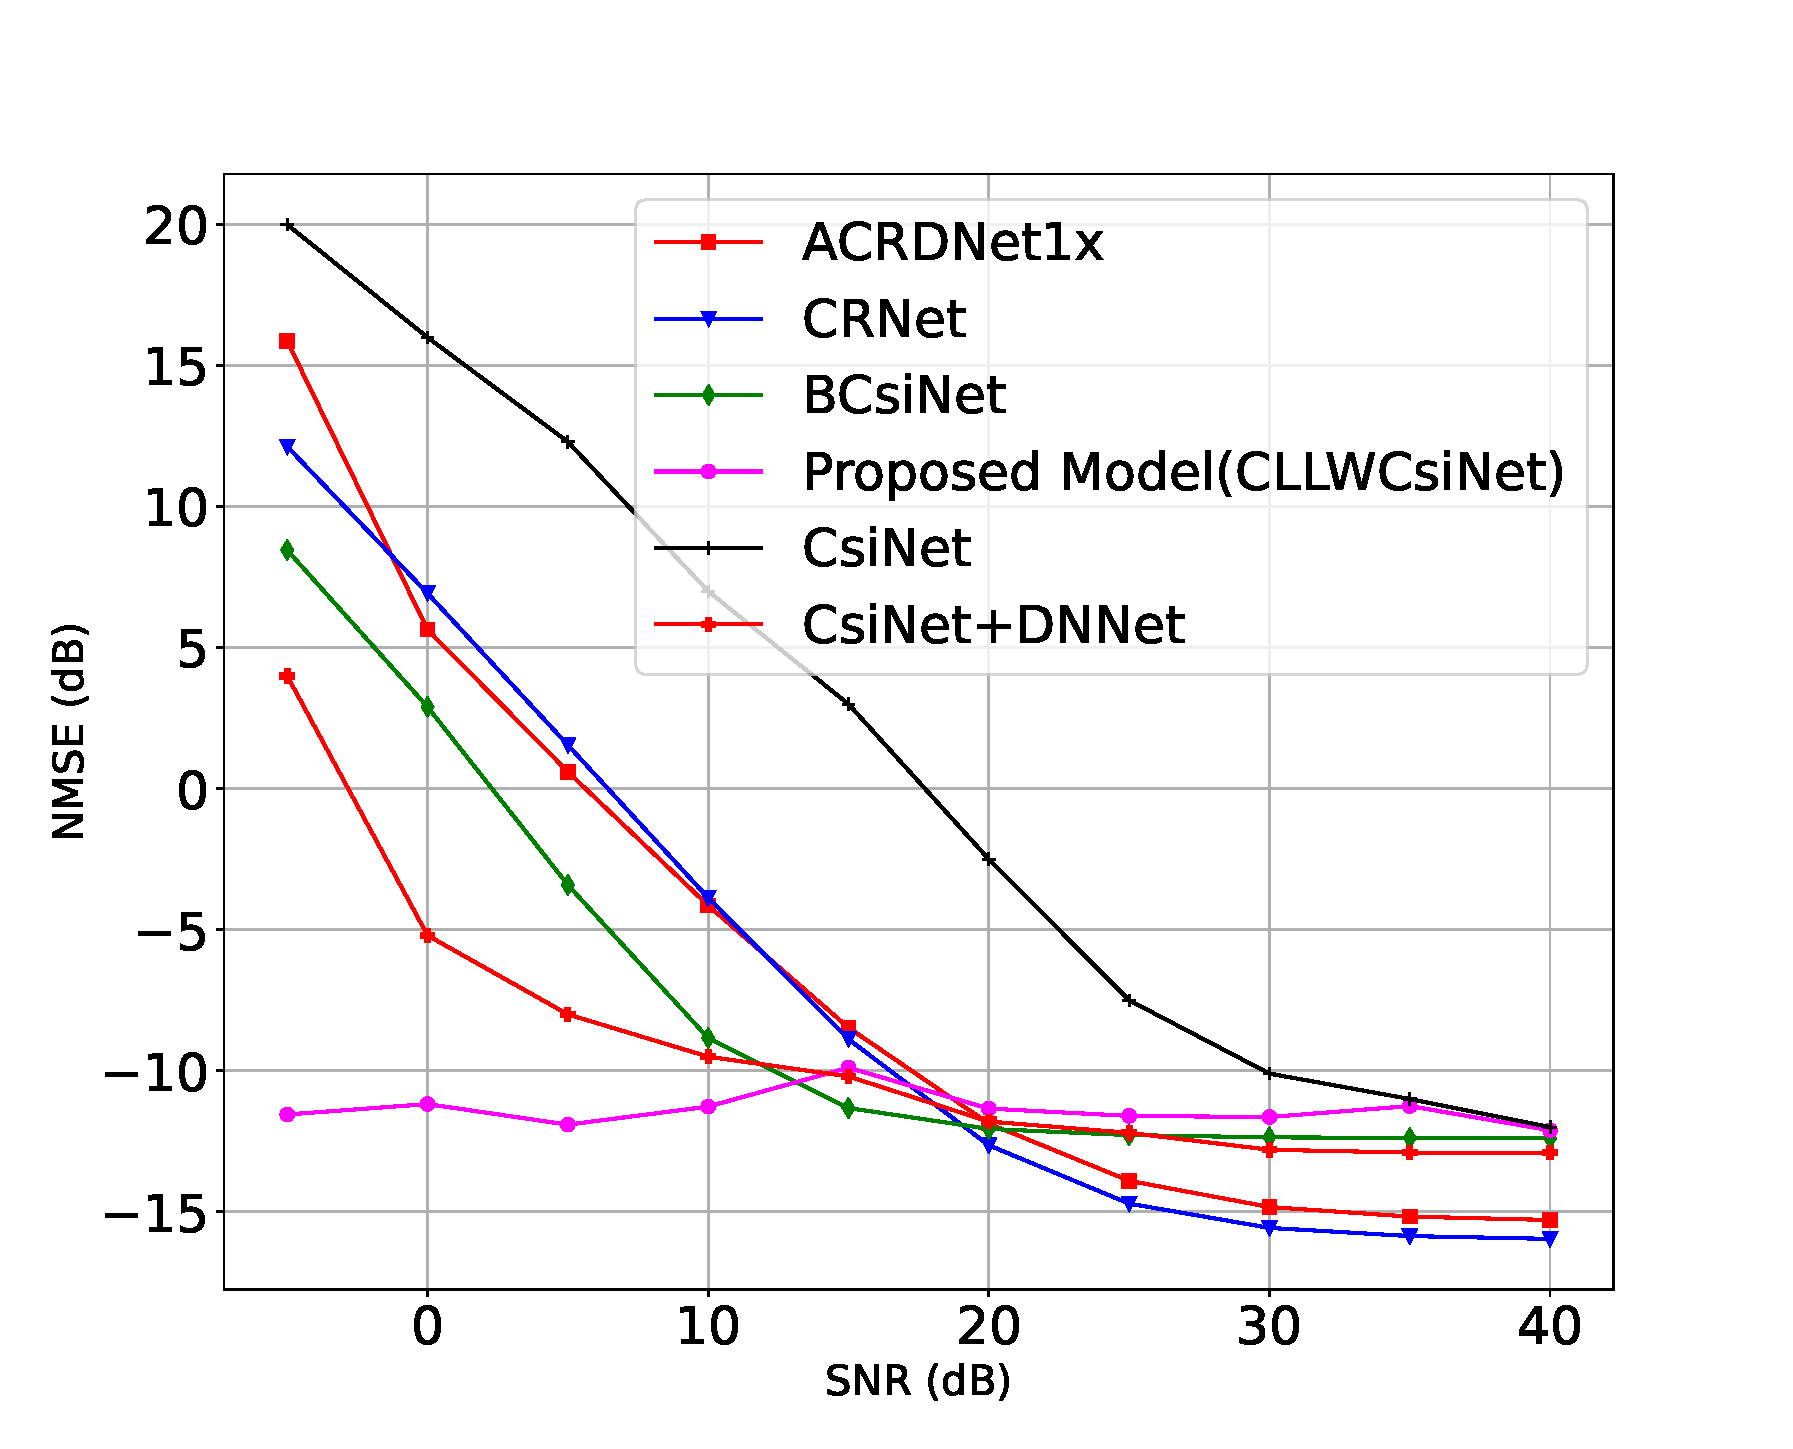
\includegraphics[width=0.53\textwidth]{Figure_1.pdf}
	\caption{Performance of Models under the various noise power and compression ratio of 8}
	\label{fig:Performance of Models under the various noise power}
\end{figure}

As illustrated in Figure \ref{fig:Performance of Models under the various noise power}, we evaluated different proposed models under various ranges of noise power, from -5 dB to 40 dB. Our proposed model outperforms previous models when the noise power is nearly greater than the signal power. Beyond 20 dB, where the signal power exceeds the noise power, CRNet \cite{abn} and ACRNet1x \cite{abx} exhibit better performance relative to our proposed model. To evaluate the previous models, we employed federated learning techniques and augmented them with additional layers to apply noise. For federated learning, we utilized the pretrained models as well. The convolutional latent space demonstrates relative correlations across various noise power levels compared to other models. Even with approximately 70K parameters, our proposed model maintains excellent performance. The proposed CLLWCsiNet model introduces innovations enhancing noise resilience and predictive accuracy, notably achieving higher correlations between successive NMSE values, making it a standout for applications requiring reliable performance in dynamic wireless environments.


\subsubsection{Convolution Factorization} To prevent an increase in FLOPs while simultaneously enhancing accuracy, we utilize convolution factorization as introduced in CRNet\cite{abn}. We employ different kernel sizes to make learning the random structure of CSI more effective. Large kernel sizes, as suggested in CsiNetPlus\cite{abo}, are used to avoid futile coefficients and ensure coverage of the CSI that contains data. Conversely, CRNet\cite{abn} suggests smaller kernel sizes for learning granular features in the CSI matrix. We integrate both approaches into a comprehensive block.

\subsubsection{Training Settings}
We trained the network for 500 epochs with a batch size of 200 and a learning rate of 0.001. The number of epochs should be carefully considered, as a high number of epochs can make the training process expensive and time-consuming for different datasets.

\subsection{Efficiency Optimization Strategies} \label{subsec:efficiency}
To address the challenges outlined in Section~\ref{sec:introduction}, CLLWCsiNet incorporates three key innovations:

\paragraph{Parameter Reduction} 
We eliminate all fully connected layers, avoiding the 2M+ parameter overhead typical in architectures like CsiNet \cite{abe} and ACRNet \cite{abx}. As demonstrated in Table~\ref{table:convlatenspacecomp}, this reduces our model to just 70K parameters while maintaining NMSE within 2 dB of FC-based designs.

\paragraph{Intelligent Kernel Selection} 
Through ablation studies, we determined that hybrid kernel sizes (combining 7×7 for global features and 3×3 for local details) provide optimal accuracy-FLOP trade-offs. This contrasts with prior work: CRNet \cite{abn} uses only small kernels, while CsiNetPlus \cite{abo} employs exclusively large ones.

\paragraph{Quantization-Aware Design} 
As shown in Table~\ref{table:dynamicquantization}, our 8-bit dynamic quantization reduces model size by 4× with $< 1\,\text{db} $ NMSE degradation. Unlike BACRNet \cite{abx} which only quantizes FC layers, we apply quantization globally, enabling deployment on CPU-only UE devices.

\begin{figure}[t]
    \centering
    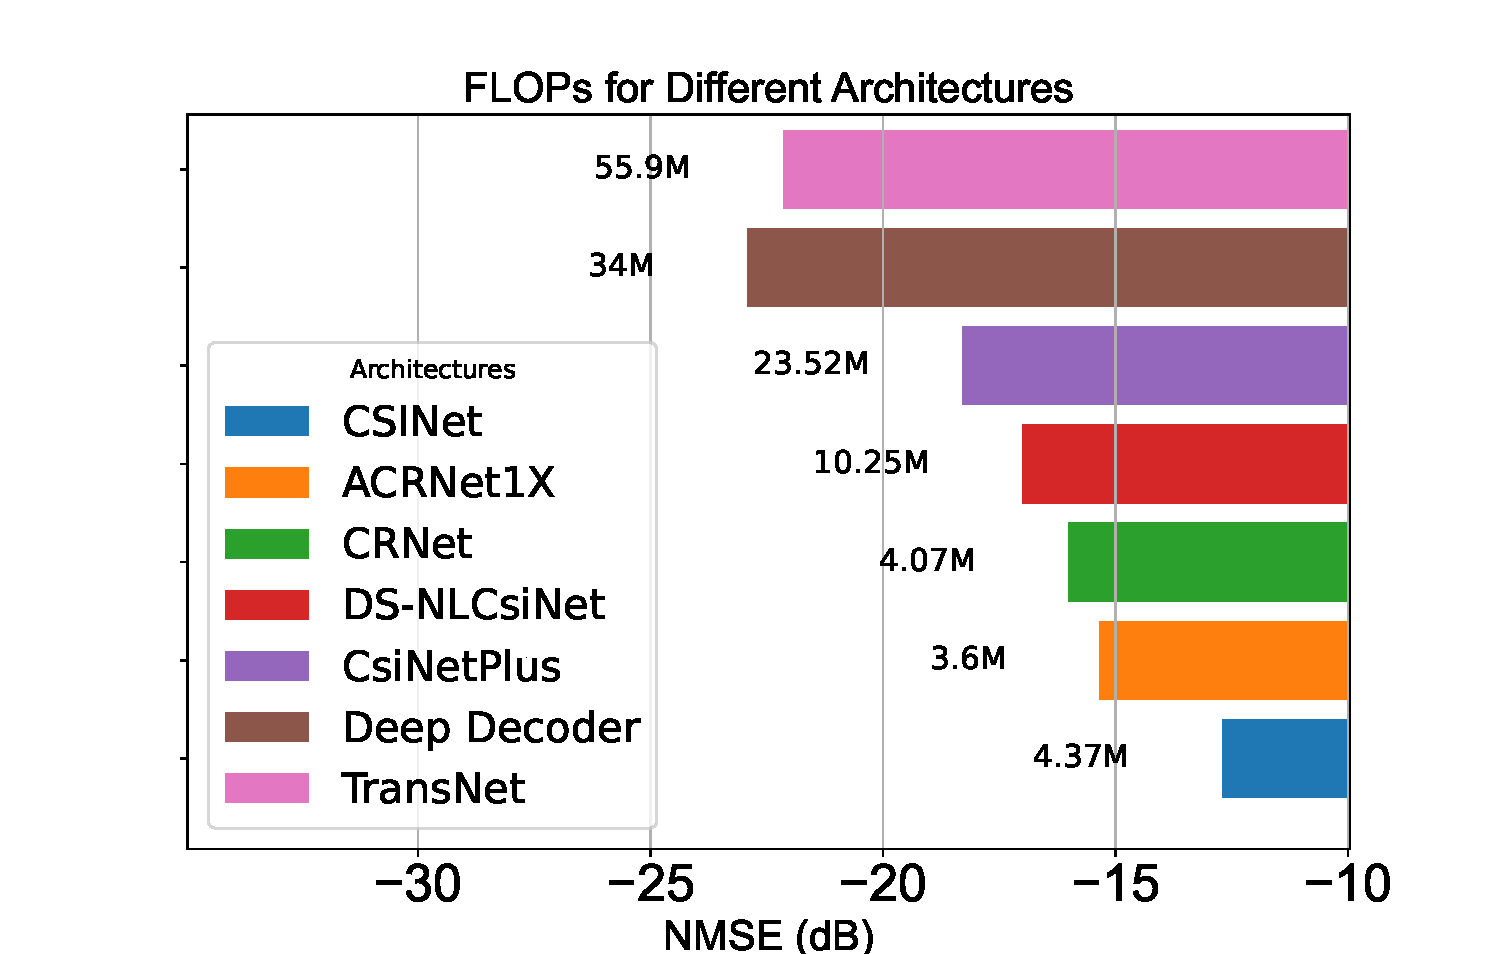
\includegraphics[width=\linewidth]{NMSEvsFLOPs.pdf}
    \caption{Our model (triangle marker) achieves better NMSE-FLOPs trade-offs than FC-heavy architectures (square markers).}
    \label{fig:efficiency-tradeoff}
\end{figure}

\subsection{Model Quantization}
Quantization is a crucial technique for optimizing deep neural networks (DNNs) to be deployed on resource-constrained devices, such as mobile phones and IoT devices. Each quantization approach offers distinct advantages and trade-offs. Neural network binarization is an extreme form of quantization where weights and activations are limited to binary values, typically -1 and 1, resulting in significant model size reduction and computational efficiency. 
\begin{equation}
	\omega_{b}=\mathrm{sign}(\omega)
\end{equation}
where \begin{math}
	\omega
\end{math}
are the original weights and \begin{math} \omega_{b}\end{math} are the binarized weights. This drastic reduction in precision requires specialized training methods to maintain accuracy. \cite{aaa1} Lu et al. \cite{abp} were pioneers in applying binary neural networks, and they later introduced vector quantization in the ACRNet\cite{abx} architecture. Their approach combined the binarization of fully connected layers with subsequent vector quantization to generate bit streams of 0s and 1s between the encoder and decoder. Convolutional quantization focuses on reducing the precision of weights and activations specifically in convolutional layers, which are prevalent in CNNs used for image processing. 
\begin{equation}
	\chi_{q}=\mathrm{round}(\frac{\chi}{S})+Z
\end{equation}
where \begin{math}
	S
\end{math} is the scale factor and \begin{math}
Z
\end{math} is the zero-point \cite{convolutionalquantization}. 
Static quantization, or post-training quantization, is performed on a pre-trained model using calibration data to determine scaling factors for weights and activations. This method reduces the precision of these elements, typically to 8-bit integers, and is suitable for deployment on fixed-resource devices with consistent input data\cite{staticquantization}.
Dynamic quantization involves quantizing weights during training and performing quantization of activations dynamically at inference time, allowing the model to adapt to varying input data distributions. This quantization process ensures that the model maintains flexibility and efficiency, adapting to different data patterns while reducing computational overhead. \cite{dynamicquantization}

In communication systems, particularly for CSI feedback from user equipment (UE) to the base station (BS), the choice of quantization method is critical. Static quantization is generally preferred for CSI feedback due to its efficiency and consistency. It provides a reliable way to map floating-point CSI values to a lower bit-width representation, typically 8-bit integers, reducing the amount of data to be transmitted without significantly affecting accuracy. This method is particularly suitable for scenarios with consistent channel conditions, allowing for effective pre-calibration.
Dynamic quantization, on the other hand, could be considered in environments with highly dynamic channel conditions where adaptability is crucial. This method allows for real-time adjustment of the quantization parameters based on the current channel state, potentially improving accuracy in dynamic environments. However, the additional computational complexity at the UE and potential latency issues need to be carefully managed.
It should be noted that all previous works have merely converted the coded sequence produced by the encoder into binary form (zeros and ones) from the perspective of a telecommunications system designer. However, for the first time, we have utilized quantization to optimize neural networks by reducing their complexity, thereby improving evaluation time and enabling implementation on telecommunications systems with limited capacity.
The NMSE reported in Table \ref{table:convlatenspacecomp} reflects the practical accuracy of the proposed models. We extend quantization to the entire network, including both neural and convolutional networks, achieving a higher NMSE compared to ACRNet, even with a significantly lower number of parameters.

\begin{figure*}[!t]
	\centering
	\begin{minipage}[b]{0.45\textwidth}
		\centering
		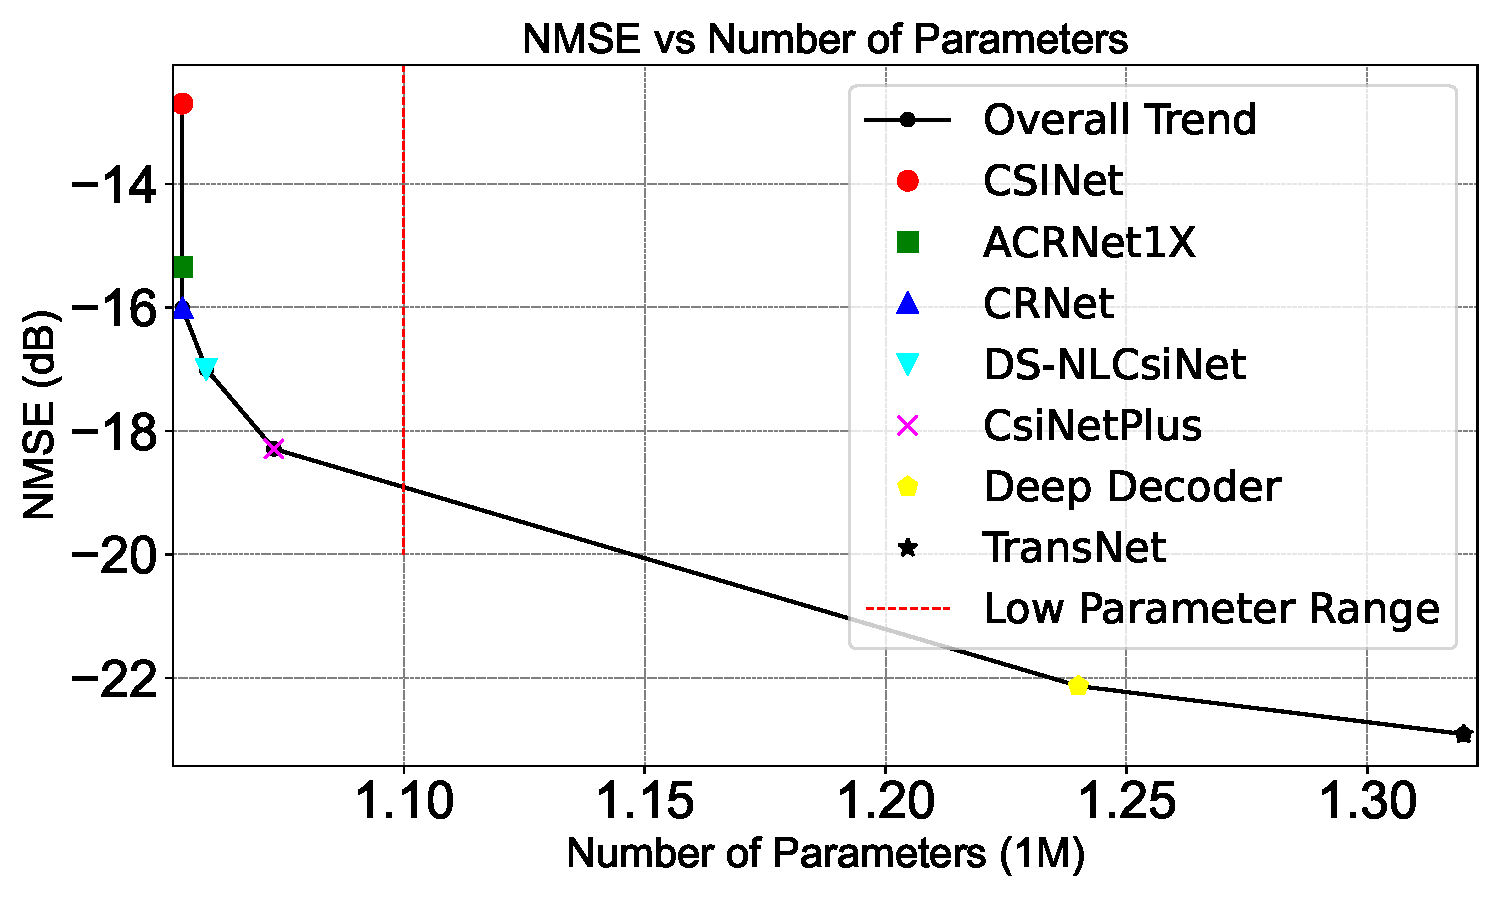
\includegraphics[width=\textwidth]{NMSEvsNofparametters.pdf}
		\caption{NMSE vs Number of Parameters}
		\label{fig:nmse-params}
	\end{minipage}
	\hfill
	
\end{figure*}

\begin{table*}[ht]
	\caption{Architecture Design for Different Compression Ratios}
	\label{table:model_comparison}
	\centering
	\begin{tabular}{cccccc}
		\toprule
		\textbf{CR} & \textbf{Code word dimension} & \textbf{Convolution Filters} & \textbf{Kernel Sizes} & \textbf{Codeword dimension} \\
		\midrule
		4 & 512 & 64, 32, 16 & $(1,7)$ & $16 \times 1 \times 32$ \\
		8 & 256 & 64, 32, 16, 8 & $(1,7)$ & $8 \times 1 \times 32$ \\
		16 & 128 & 64, 32, 16, 4 & $(1,7)$ & $4 \times 1 \times 32$ \\
		\bottomrule
	\end{tabular}
\end{table*}

\begin{table*}[ht]
	\centering
	\caption{NMSE (dB) 8-bit Dynamic Quantization of Proposed Auto-Encoders for Indoor and Outdoor Scenario}
	\label{table:dynamicquantization}
	\begin{threeparttable}
		\begin{tabular}{clcccccc}
			\toprule
			\textbf{CR} & \textbf{Architecture} & \multicolumn{2}{c}{\textbf{Indoor}} & \multicolumn{2}{c}{\textbf{Outdoor}} \\ 
			& & Params & NMSE & Params & NMSE \\ 
			\midrule
			\multirow{5}{*}{4} & BACRNet1x\cite{abx} & 71K & -14.20 & 71K & -7.03 \\  
			& QACRNet1x & 2632 & -16.19 & 2632 & -9.44 \\  
			& BCsiNet\cite{abp} & 1088K & -17.25 & 1088K & -8.35 \\ 
			& BACRNet10x\cite{abx} & 91K & \textbf{-17.27} & 91K & -8.78 \\ 
			& QACRNet10x & 23K & -13.94 & 23K & \textbf{-12.23} \\ 
			\midrule
			\multirow{5}{*}{8} & BACRNet1x\cite{abx} & 38K & -11.52 & 38K & -5.52 \\  
			& QACRNet1x & 2632 & -11.33 & 2632 & -7.20 \\  
			& BCsiNet\cite{abp} & 547K & -12.39 & 547K & -6.26 \\ 
			& BACRNet10x\cite{abx} & 58K & -14.96 & 58K & -6.63 \\ 
			& QACRNet10x & 23K & \textbf{-16.66} & 23K & \textbf{-8.57} \\ 
			\midrule
			\multirow{5}{*}{16} & BACRNet1x\cite{abx} & 7.12K & -2.19 & 21K & -2.92 \\  
			& QACRNet1x & 2632 & -9.07 & 2632 & -4.67 \\  
			& BCsiNet\cite{abp} & 276K & -8.99 & 276K & -4.11 \\ 
			& BACRNet10x\cite{abx} & 42K & -11.7 & 42K & -4.63 \\ 
			& QACRNet10x & 23K & \textbf{-12.19} & 23K & \textbf{-5.75} \\ 
			\bottomrule
		\end{tabular}
		\begin{tablenotes}
			\item[*] Q Indicates dynamic quantization based architecture 
		\end{tablenotes}
	\end{threeparttable}
\end{table*}



\begin{table*}[ht]
	\centering
	\caption{NMSE (dB) of Proposed Auto-Encoders Using Fully Connected Layers and Convolutional Latent Space for Indoor Scenario}
	\label{table:convlatenspacecomp}
	\begin{threeparttable}
		\begin{tabular}{clcccccc}
			\toprule
			\textbf{CR} & \textbf{Architecture} & \multicolumn{3}{c}{\textbf{With Conv-LatentSpace}} & \multicolumn{3}{c}{\textbf{With FC}} \\ 
			& & FLOPs & Params & NMSE & FLOPs & Params & NMSE \\ 
			\midrule
			\multirow{4}{*}{4} & CsiNet\cite{abe} & 4.00M & 17.9K & -9.72 & 5.41M & 2103K & -17.36 \\  
			& CRNet\cite{abn} & 3.72M & 17.62K & -7.35 & 5.12M & 2103K & -26.99 \\  
			& ACRNet\cite{abx} & 3.16M & 7.12K & -8.76 & 4.64M & 2102K & -27.16 \\
			& CLLWCsiNet* & 7.26M & 70.26K & \textbf{-15.09} & / & / & / \\ 
			\midrule
			\multirow{4}{*}{8} & CsiNet\cite{abe} & 3.7M & 10.71K & -3.56 & 4.37M & 1054K & -12.70 \\  
			& CRNet\cite{abn} & 3.5M & 10.43K & -4.34 & 4.07M & 1054K & -16.01 \\ 
			& ACRNet\cite{abx} & 2.93M & 9.94K & -7.72 & 3.6M & 1054K & -15.34 \\
			& CLLWCsiNet* & 7.15M & 66.7K & \textbf{-11.11} & / & / & / \\ 
			\midrule
			\multirow{4}{*}{16} & CsiNet\cite{abe} & 3.66M & 7.12K & -2.19 & 3.84M & 530K & -8.65 \\  
			& CRNet\cite{abn} & 3.38M & 6.84K & -2.49 & 3.55M & 530K & -11.35 \\ 
			& ACRNet\cite{abx} & 2.81M & 6.35K & -6.038 & 3.07M & 529K & -10.36 \\
			& CLLWCsiNet* & 6.63M & 42.6K & \textbf{-8.62} & / & / & / \\ 
			\bottomrule
		\end{tabular}
		\begin{tablenotes}[flushleft]
			\item[*] / Indicates NMSE is not reported
		\end{tablenotes}
	\end{threeparttable}
\end{table*}


\begin{figure}[ht]
	\centering
	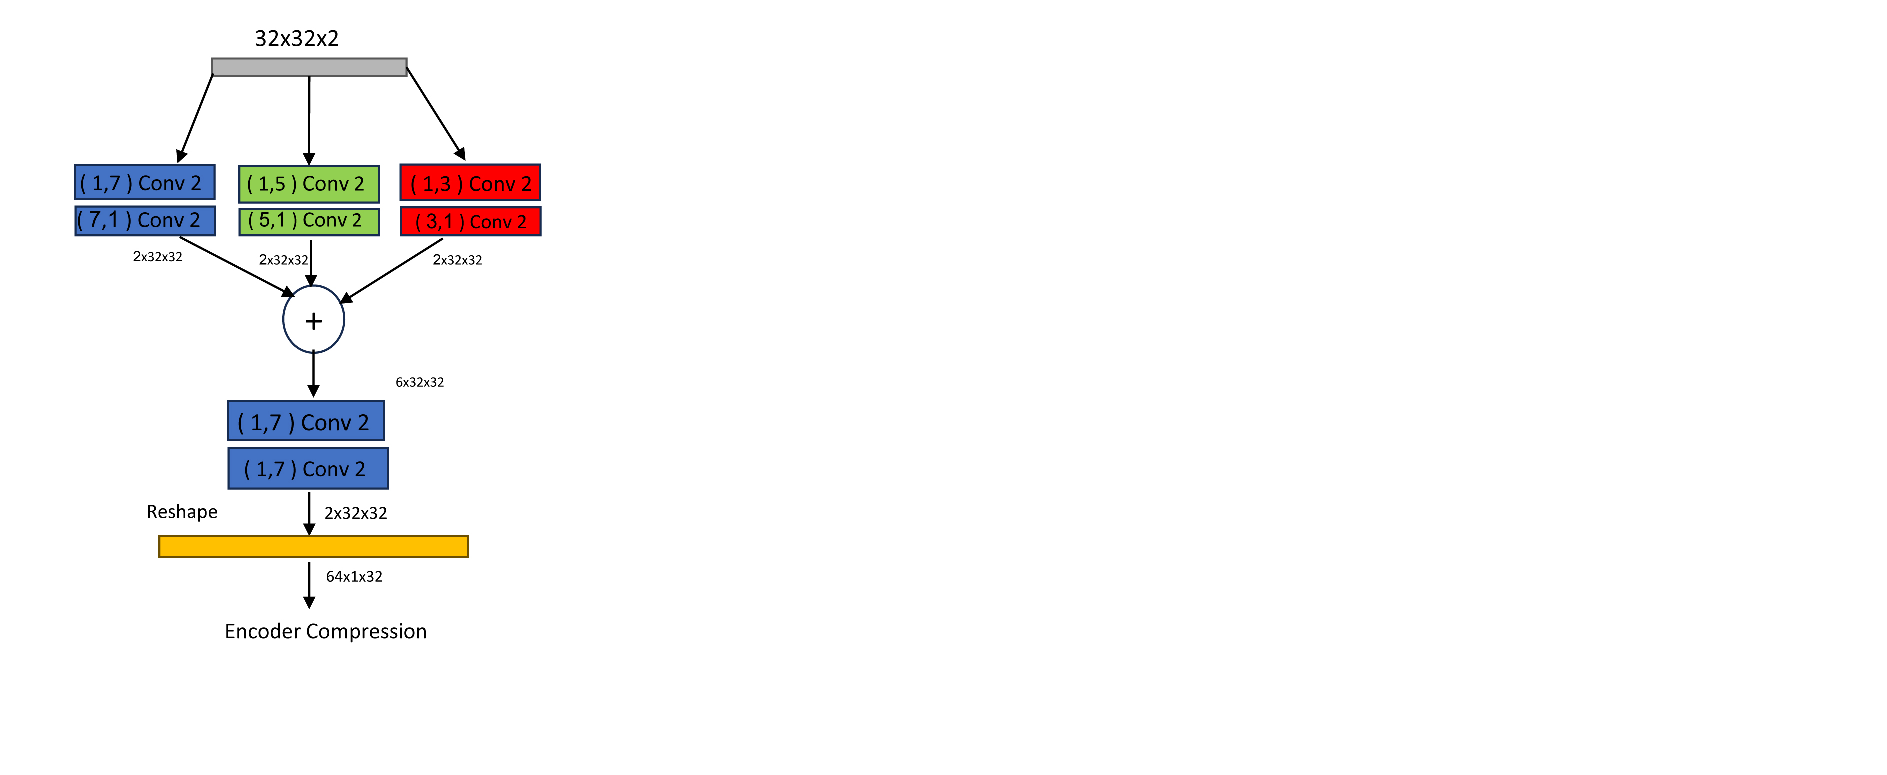
\includegraphics[width=0.6\linewidth]{Model_a.pdf}
	\caption{Encoder Architecture}
	\label{fig:figure1}
\end{figure}

\begin{figure}[ht]
	\centering
	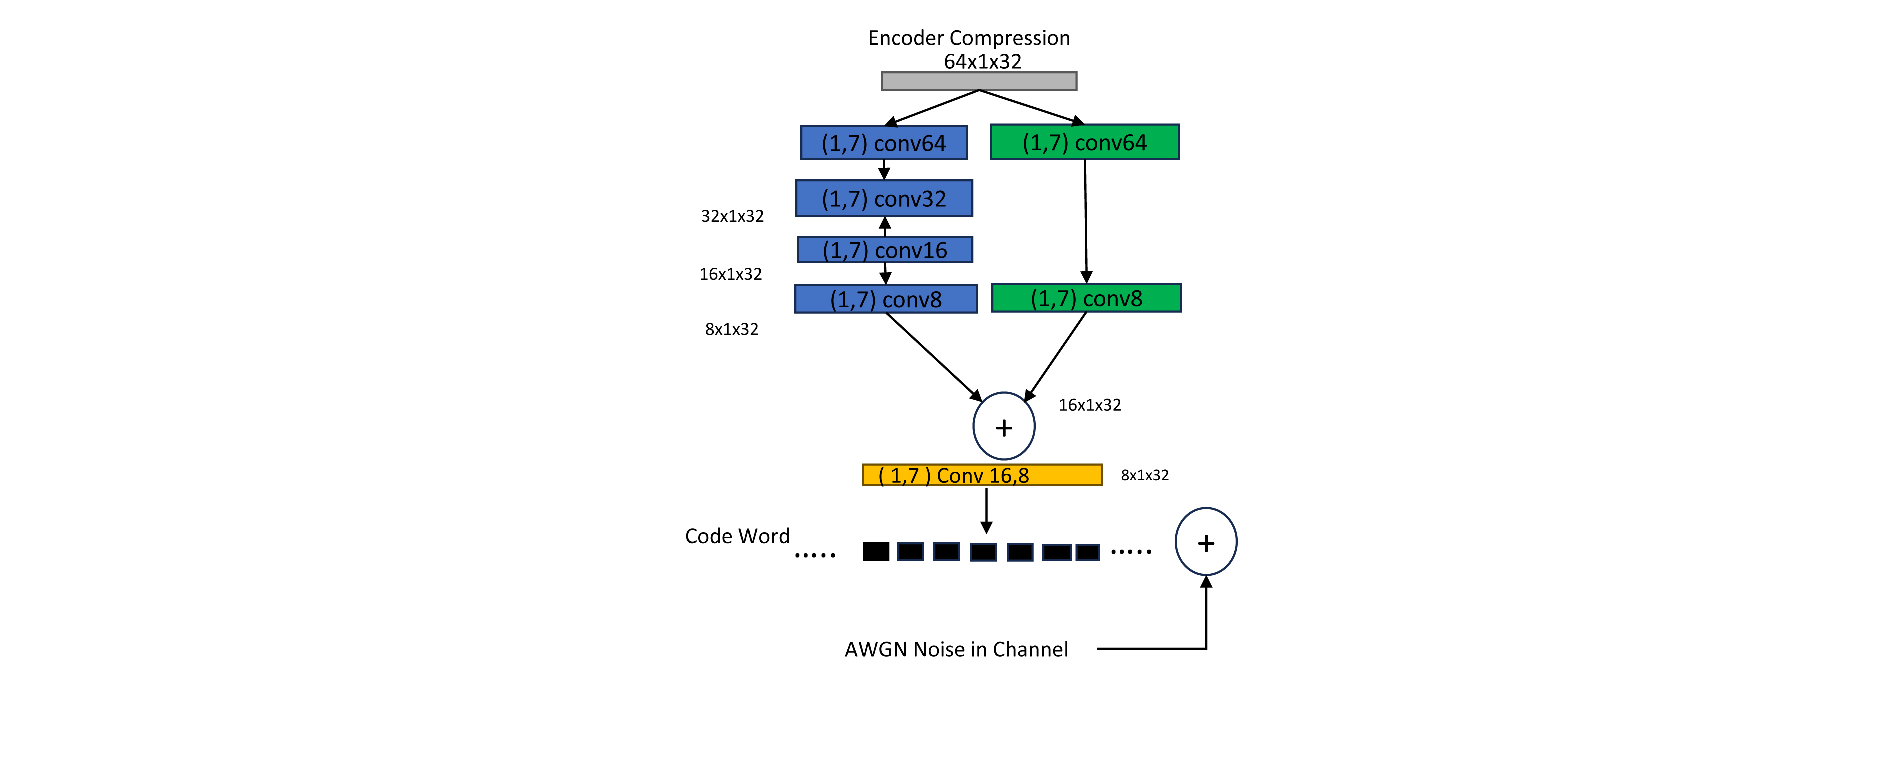
\includegraphics[width=0.8\linewidth]{Model_b.pdf}
	\caption{Convolutional Latent-Space}
	\label{fig:figure2}
\end{figure}

\begin{figure}[ht]
	\centering
	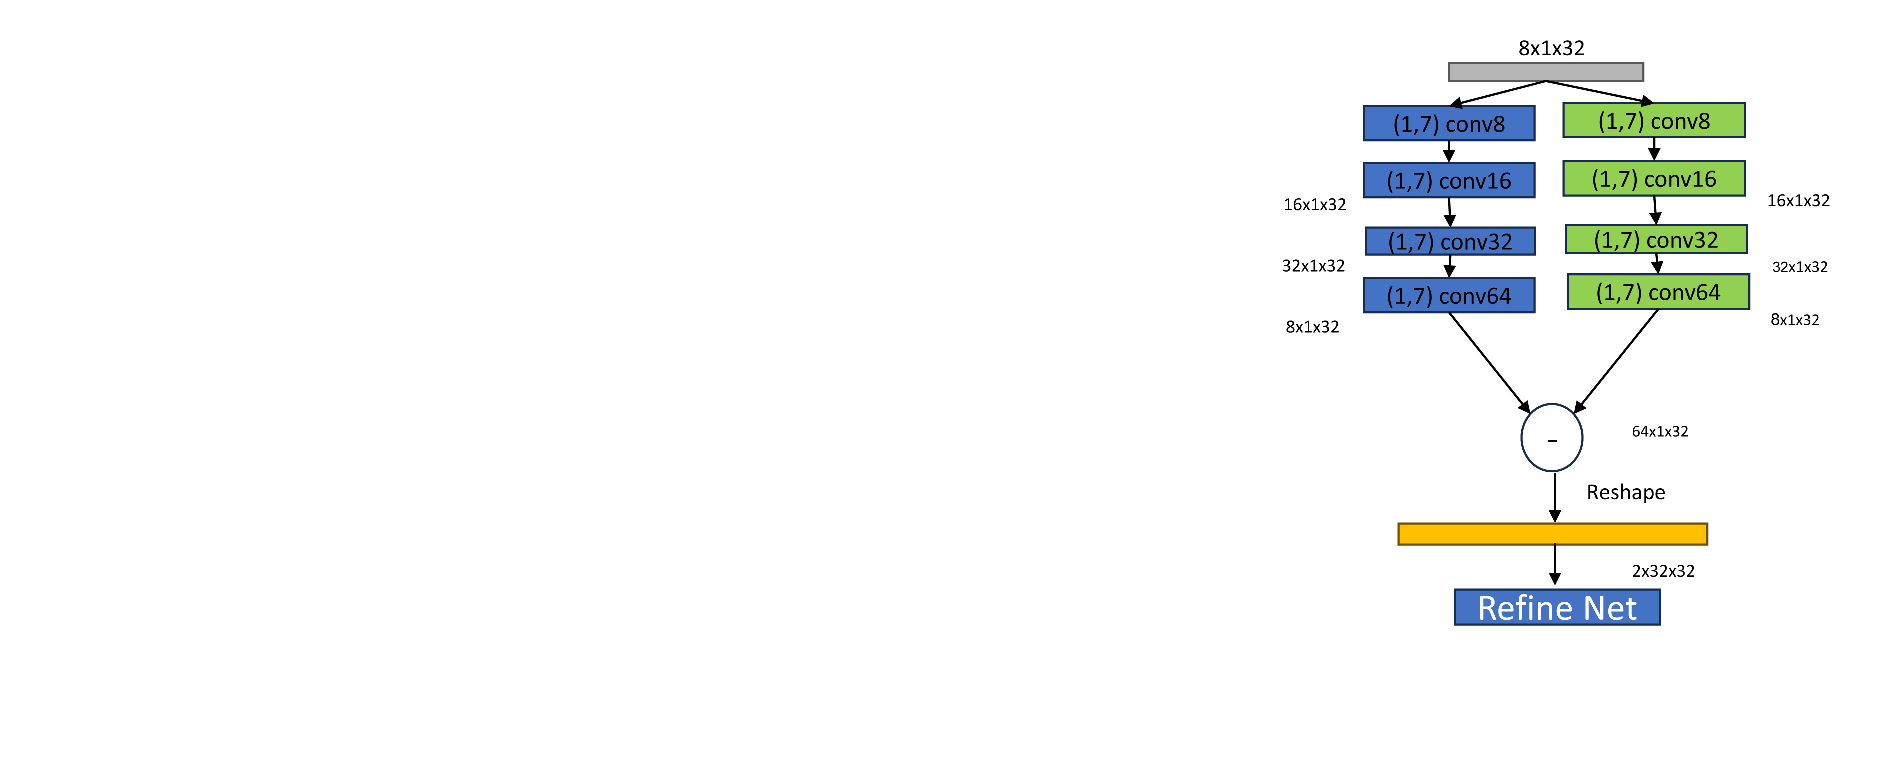
\includegraphics[width=0.8\linewidth]{Model_c.pdf}
	\caption{Denoising Module and Refinement}
	\label{fig:figure3}
\end{figure}



	
	\begin{table*}[ht]
		\centering
		\caption{Performance Comparison for 3GPP 38.901 UMa NLOS Channel Model at CR=4 for Outdoor Scenario}
		\label{table:performance_comparison}
		\begin{threeparttable}
			\begin{tabular}{cccc}
				\toprule
				\textbf{Frequency} & \textbf{Model} & \textbf{NMSE (dB) Quadriga} & \textbf{NMSE (dB) COST2100} \\
				\midrule
				\multirow{4}{*}{28 GHz} & ACRNet1x\cite{abx} & -0.09 & - \\
				& CRNet\cite{abn} & 1.22 & - \\
				& BCsiNet\cite{abp} & 1.33 & - \\
				& CLLWCsiNet* & 0.08 & - \\
				\midrule
				\multirow{4}{*}{300 MHz} & ACRNet1x\cite{abx} & 0.55 & -10.71 \\
				& CRNet\cite{abn} & 1.31 & -12.70 \\
				& BCsiNet\cite{abp} & 1.61 & -8.35 \\
				& CLLWCsiNet* & 0.008 & -7.89 \\
				\bottomrule
			\end{tabular}
			\begin{tablenotes}
				\item[*] $ -$ Indicates NMSE is not reported
				\item[*] $ *$ Proposed Model
			\end{tablenotes}
		\end{threeparttable}
	\end{table*}
	




\section{Model Generalization}


Our work assumes Rayleigh fading for the system model but trains on COST 2100 data, which introduces a discrepancy between the idealized channel and the realistic training environment. While this approach provides a tractable baseline, future work should align the system model with geometry-based channel models (e.g., COST 2100 or 3GPP TR 38.901) to fully capture spatial correlations and frequency-dependent effects in end-to-end simulations.

Most research on CSI compression through deep learning employs the COST2100 channel model for both indoor and outdoor scenarios, specifically at 5.3 GHz for indoor and 300 MHz for outdoor scenarios. However, an important question arises: will these proposed models be successful on other channel models?
\cite{abn} state that overfitting is rare in the construction of CSI feedback matrices, presenting two primary reasons. First, the number of FLOPs is relatively low compared to the large models used in image processing. Second, the structure of the CSI feedback matrix is unique. \cite{abx} discuss the random structure of CSI feedback, which complicates the learning process due to the lack of common patterns in the feedback.

To the best of our knowledge, this is the first time the proposed models have been tested on the Quadriga dataset for an outdoor scenario at 300 MHz and 28 GHz mmWaves. As shown in Table
 \ref{table:performance_comparison}, state-of-the-art models fail to reconstruct the CSI feedback accurately, indicating potential overfitting of the proposed models on the COST2100 dataset. To address this, we employ the 3GPP 38.901 UMa NLOS channel model using the Quadriga software. We generate 20,000 samples to test the trained model through federated learning. To the best of our knowledge, this is the first research to test the proposed models on a different dataset to generalize the models. We separate the real and imaginary parts of the CSI matrices generated in the angular-delay domain.

We employed the 3GPP 38.901 UMa NLOS channel model at two different frequencies. We evaluated some state-of-the-art models on the mmWave 2.8 GHz frequency band using 13,000 samples for the outdoor scenario. The second setting is at 5.3 GHz, with UE mobility of 0.9 meters per second, a setting similar to the COST2100 channel model for outdoor scenarios. This allows us to determine whether the proposed models are overfitting to the COST2100 channel model, an important consideration that has been largely neglected in most previous research. We use the saved checkpoints reported by some studies to generate their results.

    

	
\begin{figure}[ht]
		\centering
		\subfloat[]{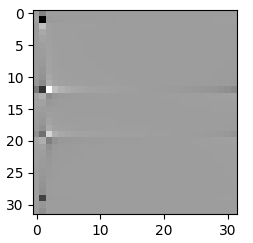
\includegraphics[width=2.5cm]{2.8_1}}%
		\hfill
		\subfloat[]{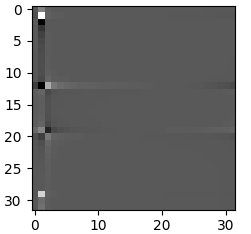
\includegraphics[width=2.5cm]{2.8_2}}%
		\hfill
		\subfloat[]{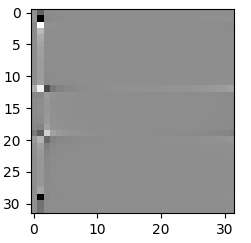
\includegraphics[width=2.5cm]{2.8-3}}%
		\caption{CSI Feedback of Quadriga channel model for Outdoor scenario 28GHz.}
		\label{fig:quadriga_28ghz}
	\end{figure}
	
	\begin{figure}[ht]
		\centering
		\subfloat[]{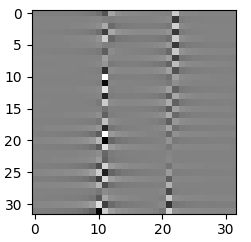
\includegraphics[width=2.5cm]{5.3_1}}%
		\hfill
		\subfloat[]{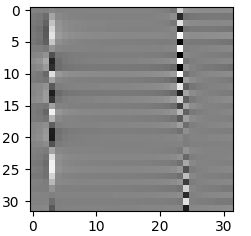
\includegraphics[width=2.5cm]{5.3_2}}%
		\hfill
		\subfloat[]{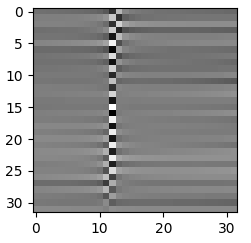
\includegraphics[width=2.5cm]{5.3_3}}%
		\caption{CSI Feedback of Quadriga channel model for Outdoor scenario 300MHz.}
		\label{fig:quadriga_300mhz}
	\end{figure}
	
	\begin{figure}[ht]
		\centering
		\subfloat[]{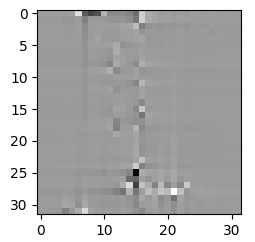
\includegraphics[width=2.5cm]{C2100_1_out}}%
		\hfill
		\subfloat[]{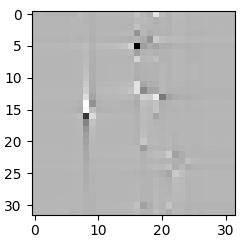
\includegraphics[width=2.5cm]{C2100_2_out}}%
		\hfill
		\subfloat[]{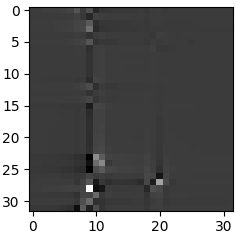
\includegraphics[width=2.5cm]{C2100_3_out}}%
		\caption{CSI Feedback of COST2100 channel model for Outdoor scenario 300MHz.}
		\label{fig:cost2100_300mhz}
	\end{figure}
	









The table \ref{table:performance_comparison} illustrates a notable decline in performance among the models when evaluating the channel state information generated by Quadriga models. This observation suggests a clear instance of overfitting.

TABLE \ref{table:performance_comparison} evaluates four models (ACRNet, CRNet, BCsiNet, CLLWCsiNet) for their suitability in outdoor communication systems operating at 28 GHz and 300 MHz. Based on NMSE for data sets (Quadriga, COST2100), CLLWCsiNet appears to outperform the other models at both frequencies, followed by ACRNet and CRNet while other models evaluate in perfect channel, CLLWCsiNet has been consider under 40db SNR.


\section{Conclusion}
In this work, we introduced CLLWCsiNet, a novel deep learning model tailored for compressing CSI feedback in MIMO systems under 5G and 6G network constraints. CLLWCsiNet utilizes convolutional latent-space compression to significantly reduce parameters while maintaining high predictive accuracy, making it suitable for resource-limited user equipment. By integrating noise resilience and a denoising network, our model demonstrates robust performance in noisy channel conditions, crucial for reliable CSI reconstruction.
Evaluation across diverse channel models, including Quadriga datasets at various frequencies, highlighted CLLWCsiNet's superior performance over existing models like ACRNet and CRNet. This underscores its potential to generalize beyond the COST2100 dataset, mitigating overfitting concerns observed in previous studies. Additionally, we explored static and dynamic quantization techniques tailored for efficient deployment in wireless communication systems. Dynamic quantization emerged as a promising approach, adapting to dynamic channel conditions while maintaining computational efficiency. In conclusion, CLLWCsiNet represents a significant advancement in CSI compression for MIMO systems, offering a balanced solution of accuracy and efficiency in challenging wireless environments. Future research will focus on optimizing architectures for heterogeneous networks and refining quantization strategies for broader deployment scenarios.

\begin{thebibliography}{00}
    \bibitem{abc} 
    Lu, L., et al. "An Overview of Massive MIMO: Benefits and Challenges," in IEEE Journal of Selected Topics in Signal Processing, vol. 8, no. 5, pp. 742-758, 2014.

    \bibitem{abd} 
    T. Marzetta. "Noncooperative Cellular Wireless with Unlimited Numbers of Base Station Antennas," in IEEE Transactions on Wireless Communications, vol. 9, no. 11, pp. 3590-3600, 2010.

    \bibitem{vectorquantiz} 
    David James Love, undefined., et al. "An overview of limited feedback in wireless communication systems," in IEEE Journal on Selected Areas in Communications, vol. 26, 2008.

    \bibitem{pca} 
    Zhu, Z., et al, "Asymmetric Non-Local Neural Networks for Semantic Segmentation," in 2019 IEEE/CVF International Conference on Computer Vision (ICCV), 2019, pp. 593-602.

    \bibitem{compressivesensing} 
    P. Kuo, H. Kung, P. Ting, "Compressive sensing based channel feedback protocols for spatially-correlated massive antenna arrays," in 2012 IEEE Wireless Communications and Networking Conference (WCNC), 2012, pp. 492-497.

    \bibitem{abe} 
    C. Wen, W. Shih, S. Jin. "Deep Learning for Massive MIMO CSI Feedback," in IEEE Wireless Communications Letters, vol. 7, no. 5, pp. 748-751, 2018.

    \bibitem{abf} 
    Liu, L., et al. "The COST 2100 MIMO channel model," in IEEE Wireless Communications, vol. 19, pp. 92-99, 2012.

    \bibitem{abg} 
    He, K., et al, "Deep Residual Learning for Image Recognition," in 2016 IEEE Conference on Computer Vision and Pattern Recognition (CVPR), 2016, pp. 770-778.

    \bibitem{abh} 
    Tianqi Wang, et al. "Deep Learning-based CSI Feedback Approach for Time-varying Massive MIMO Channels," in CoRR, vol. abs/1807.11673, 2018.

    \bibitem{abi} 
    Lu, C., et al. "MIMO Channel Information Feedback Using Deep Recurrent Network," in IEEE Communications Letters, vol. 23, no. 1, pp. 188-191, 2019.

    \bibitem{mashhadi2020deepcmc} 
    M.~B.~Mashhadi, Q.~Yang, and D.~Gunduz, ``Distributed deep convolutional compression for massive MIMO CSI feedback,'' \textit{IEEE Trans. Wireless Commun.}, vol.~19, no.~8, pp.~5317--5328, Aug.~2020.

    \bibitem{shehzad2021design} 
    M. K. Shehzad, L. Rose, S. Wesemann, M. Assaad, and S. A. Hassan, ``Design of an Efficient CSI Feedback Mechanism in Massive MIMO Systems: A Machine Learning Approach using Empirical Data,'' arXiv preprint arXiv:2208.11951v1, 2021.

    \bibitem{zhang2022quantization} 
    X. Zhang, Z. Lu, R. Zeng, and J. Wang, ``Quantization Adaptor for Bit-Level Deep Learning-Based Massive MIMO CSI Feedback,'' arXiv preprint arXiv:2211.02937v2, 2022.

    \bibitem{liu2023continuous} 
    Y. Liu et al., ``Continuous Online Learning-Based CSI Feedback in Massive MIMO Systems,'' \textit{IEEE Wireless Commun. Lett.}, early access, 2023, doi: 10.1109/LWC.2023.10381825.

    \bibitem{guo2023ris} 
    J. Guo, X. Yang, C.-K. Wen, S. Jin, and G. Y. Li, ``Deep learning-based CSI feedback for RIS-assisted multi-user systems,'' \textit{arXiv preprint arXiv:2003.03303}, 2023.

    \bibitem{abj} 
    X. Li, H. Wu. "Spatio-Temporal Representation With Deep Neural Recurrent Network in MIMO CSI Feedback," in IEEE Wireless Communications Letters, vol. 9, no. 5, pp. 653-657, 2020.

    \bibitem{abk} 
    Z. Liu, M. Rosario, Z. Ding. "A Markovian Model-Driven Deep Learning Framework for Massive MIMO CSI Feedback," in IEEE Transactions on Wireless Communications, vol. 21, no. 2, pp. 1214-1228, 2022.

    \bibitem{abn} 
    Zhilin Lu, Jintao Wang, Jian Song. "Multi-resolution CSI Feedback with Deep Learning in Massive MIMO System," in ICC 2020 - 2020 IEEE International Conference on Communications (ICC), pp. 1-6, 2019.

    \bibitem{abo} 
    Jiajia Guo, et al. "Convolutional Neural Network-Based Multiple-Rate Compressive Sensing for Massive MIMO CSI Feedback: Design, Simulation, and Analysis," in IEEE Transactions on Wireless Communications, vol. 19, pp. 2827-2840, 2019.

    \bibitem{abq} 
    Yu, X., et al. "DS-NLCsiNet: Exploiting Non-Local Neural Networks for Massive MIMO CSI Feedback," in IEEE Communications Letters, vol. 24, no. 12, pp. 2790-2794, 2020.

    \bibitem{abr} 
    Zhu, Z., et al, "Asymmetric Non-Local Neural Networks for Semantic Segmentation," in 2019 IEEE/CVF International Conference on Computer Vision (ICCV), 2019, pp. 593-602.

    \bibitem{abs} 
    Q. Cai, C. Dong, K. Niu, "Attention Model for Massive MIMO CSI Compression Feedback and Recovery," in 2019 IEEE Wireless Communications and Networking Conference (WCNC), 2019, pp. 1–5.

    \bibitem{abt} 
    J. Hu, L. Shen, G. Sun, "Squeeze-and-excitation networks," in Proceedings of the IEEE conference on computer vision and pattern recognition, 2018, pp. 7132–7141.

    \bibitem{abm} 
    G. Jiajia, C. Wen, S. Jin. "Deep Learning-Based CSI Feedback for Beamforming in Single-and Multi-cell Massive MIMO Systems," in IEEE Journal on Selected Areas in Communications, 2021.

    \bibitem{abp} 
    Z. Lu, J. Wang, J. Song. "Binary Neural Network Aided CSI Feedback in Massive MIMO System," in IEEE Wireless Communications Letters,, 2020.

    \bibitem{wang2024better} 
    J. Wang et al., ``Toward Better Low-Rate DL-Based CSI Feedback: A Test Channel-Based Approach,'' \textit{IEEE Trans. Wireless Commun.}, vol. 23, no. 5, pp. 3210-3224, May 2024.

    \bibitem{zhang2024zone} 
    Y. Zhang, A. Alkhateeb, ``Zone-Specific CSI Feedback for Massive MIMO,'' \textit{IEEE Wireless Commun. Lett.}, early access, 2024.

    \bibitem{chen2024transnet} 
    Q. Chen, A. Guo, and Y. Cui, ``Multi-head transformer architecture for massive MIMO CSI feedback,'' \textit{Appl. Sci.}, vol. 14, no. 3, p. 1356, 2024.

    \bibitem{li2024lightweight} 
    X. Li, Y. Wang, and Z. Zhang, ``A lightweight design to convolution-based deep learning CSI feedback,'' \textit{IEEE Wireless Commun. Lett.}, 2024.

    \bibitem{wang2024variational} 
    Y. Wang et al., ``Enhancing deep learning-based CSI feedback in noisy channels with a soft variational approach,'' \textit{IEEE Trans. Wireless Commun.}, early access, 2024.

    \bibitem{Ma2024} 
    Y. Ma, H. He, S. Song, J. Zhang, and K. B. Letaief, ``Low-Complexity CSI Feedback for FDD Massive MIMO Systems via Learning to Optimize,'' \textit{arXiv preprint arXiv:2406.16323}, 2024.

    \bibitem{prac2024} 
    Z. Lu, Y. Dong, H. He, S. Jin, and G. Y. Li, ``Practical Deployment for Deep Learning-Based CSI Feedback Systems: Generalization Challenges and Enabling Techniques,'' \textit{IEEE Wireless Communications}, vol. 31, no. 2, pp. 72--79, Apr. 2024, doi: 10.1109/MWC.001.2300223.

    \bibitem{quant2024} 
    M. Yin, S. Han, and C. Yang, ``Quantization Design for Deep Learning-Based CSI Feedback,'' \textit{arXiv preprint arXiv:2503.08125}, Mar. 2024.

    \bibitem{CSICompression2024} 
    J.~Chen, W.~J.~Hillery, K.~R.~Mestav, C.~Nuzman, I.~Saniee, and Y.~Xing, ``CSI Compression for Massive MIMO: Model-Based or Data-Driven?,'' \emph{IEEE Wireless Communications}, vol.~32, no.~1, pp.~22--27, Feb. 2025.

    \bibitem{Guo2024} 
    Y. Guo, W. Chen, F. Sun, J. Cheng, M. Matthaiou, and B. Ai, ``Deep Learning for CSI Feedback: One-Sided Model and Joint Multi-Module Learning Perspectives,'' \textit{arXiv preprint arXiv:2405.05522}, 2024.

    \bibitem{abw} 
    Hongyuan Ye, undefined., et al. "Deep Learning-Based Denoise Network for CSI Feedback in FDD Massive MIMO Systems," in IEEE Communications Letters, vol. 24, pp. 1742-1746, 2020.

    \bibitem{abx} 
    Lu, Z., et al. "Binarized Aggregated Network With Quantization: Flexible Deep Learning Deployment for CSI Feedback in Massive MIMO Systems," in IEEE Transactions on Wireless Communications, vol. 21, no. 7, pp. 5514-5525, 2022.

    \bibitem{ji2021clnet} 
    S. Ji and M. Li, ``CLNet: Complex input lightweight neural network designed for massive MIMO CSI feedback,'' \textit{IEEE Wireless Commun. Lett.}, vol. 10, no. 10, pp. 2318--2322, Oct. 2021.

    \bibitem{aby} 
    Chakma, A., et al. "Deep Decoder CsiNet for FDD Massive MIMO System," in IEEE Wireless Communications Letters, vol. 12, no. 12, pp. 2073-2077, 2023.

    \bibitem{abz} 
    Y. Cui, A. Guo, C. Song. "TransNet: Full Attention Network for CSI Feedback in FDD Massive MIMO System," in IEEE Wireless Communications Letters, vol. 11, no. 5, pp. 903-907, 2022.

    \bibitem{abu} 
    Burkhardt, F., et al, "QuaDRiGa: A MIMO channel model for land mobile satellite," in The 8th European Conference on Antennas and Propagation (EuCAP 2014), 2014, pp. 1274-1278.

    \bibitem{aaa1} 
    Markus Nagel, Marios Fournarakis, Rana Ali Amjad, Yelysei Bondarenko, Mart van Baalen, Tijmen Blankevoort (2021). A White Paper on Neural Network Quantization. ArXiv, abs/2106.08295.

    \bibitem{ccc1} 
    Zhang, K., et al. "Beyond a Gaussian Denoiser: Residual Learning of Deep CNN for Image Denoising," in IEEE Transactions on Image Processing, vol. 26, no. 7, pp. 3142-3155, 2017.

    \bibitem{quantization} 
    Markus Nagel, undefined., et al. "A White Paper on Neural Network Quantization," in ArXiv, vol. abs/2106.08295, 2021.

    \bibitem{convolutionalquantization} 
    Y. Chenna. "Quantization of Convolutional Neural Networks: A Practical Approach," in International Journal of Recent Technology and Engineering (IJRTE), vol. 8, 2023.

    \bibitem{staticquantization} 
    S. Han, H. Mao, and W. J. Dally, "Quantizing deep convolutional networks for efficient inference: A whitepaper," arXiv preprint arXiv:1512.02572, 2015.

    \bibitem{dynamicquantization} 
    Y. Zhou, S. Liu, J. Wang, Y. Eiss, X. Huang, and E. Elsen, "Efficient 8-bit quantization of Transformer neural machine language translation model," arXiv preprint arXiv:2006.16669, 2020.
\end{thebibliography}



\end{document}


